\documentclass[11pt]{report}
%\usepackage[margin=0.625in]{geometry}
%\usepackage{blindtext}
%\usepackage{setspace}
%\usepackage[english]{babel}
%\usepackage{indentfirst}
\usepackage{amssymb}
\usepackage{amsmath}
\usepackage{breqn}
\usepackage{graphics}
\usepackage{comment}
\usepackage{latexsym}
\usepackage{setspace}
\usepackage{multicol}
\usepackage[T1]{fontenc}
\usepackage[ruled, linesnumbered]{algorithm2e}
%\RestyleAlgo{ruled}
\usepackage{graphicx}
\usepackage{caption}
\usepackage[table,xcdraw]{xcolor}
\usepackage{booktabs}
\usepackage{tikz}
\usepackage{parskip}
\usepackage{pgfplots}
\usepackage{hyperref}
\hypersetup{
    colorlinks=true,
    linkcolor=blue,
    filecolor=blue,      
    urlcolor=blue,
    citecolor=blue,
    pdftitle={The CUDA Parallel Programming API and Workflow},
    pdfpagemode=FullScreen,
}
\usepackage{float}
\usepackage{csquotes}
\usepackage[
backend=biber,
style=numeric,
sorting=ynt
]{biblatex}

\setlength{\oddsidemargin}{0.0in}
\setlength{\marginparsep}{0pt}
\setlength{\marginparwidth}{0pt}
\setlength{\textwidth}{6.5truein}
\setlength{\voffset}{-1.0in}
\setlength{\textheight}{700pt}


\pgfplotsset{compat=1.18}


\addbibresource{bib.bib}

%\doublespacing
\begin{document}

\begin{titlepage}
   \begin{center}
       \vspace*{1cm}

        {\Huge
       \textbf{Parallel Computing Paradigms: Exploring CUDA Methodology and Workflow for Combinatorial Optimization}

       \vspace{0.5cm}}
        Leveraging CUDA for High-Performance Computing and GPU-Driven Optimization
            
       \vspace{1.5cm}

       \textbf{Andrew Struthers, Hunter Lawrence}\\
       April 25, 2024

       \vfill
            
       CS 530: High Performance Computing\\
       Dr. Szil\'ard VAJDA
            
       \vspace{0.8cm}
       
\includegraphics[width=0.8\textwidth]{Images/university_logo}
            
       Department of Computer Science\\
       Central Washington University\\
       Ellensburg, WA, United States of America\\
       Spring Quarter, 2024
            
   \end{center}
\end{titlepage}


\section*{Abstract}
In the realm of high-performance computing, the use of Graphics Processing Units (GPUs) has revolutionized the landscape of parallel computing. This report delves into the integration of CUDA (Compute Unified Device Architecture)—NVIDIA's parallel computing platform and application programming interface—within the domain of combinatorial optimization.

The report begins with an in-depth exploration of CUDA, covering its evolution, programming model, performance optimizations, and diverse applications across scientific simulations, deep learning, and industrial domains. Subsequently, the focus shifts towards combinatorial optimization, outlining classical algorithms and their adaptation for parallel execution on GPUs.

The methodology section discusses the setup of CUDA development environments, design considerations for parallel optimization algorithms, and the seamless integration of CUDA with combinatorial problem domains. Through a series of case studies, including the Traveling Salesman Problem and graph coloring algorithms, we demonstrate the efficacy of CUDA in accelerating solution times and scaling to large problem sizes.

Results and analysis present detailed performance metrics, benchmarking results, and comparisons with traditional CPU-based approaches, highlighting the tangible benefits of GPU acceleration for combinatorial optimization tasks. Challenges such as scalability and future research directions are also discussed, underscoring the ongoing pursuit of optimizing CUDA for complex combinatorial problems.

Overall, this report\footnote{This report is organized in such a way where Chapter 1, 2, 3, and 4 are capable of standing alone outside of the structure of the entire report. As such, some information might be repeated in places where a reminder or a refresher might be useful.} provides a comprehensive examination of the intersection between CUDA and combinatorial optimization, offering insights into the potential of GPU-driven parallel computing to drive innovation in optimization algorithms and real-world applications.



\addcontentsline{toc}{section}{Abstract}

\tableofcontents
%\doublespacing
\chapter{Introduction to CUDA}
Compute Unified Device Architecture (CUDA) was released as an Application Programming Interface (API) by the NVIDIA Corporation in 2006\cite{CPP_GUIDE} to allow programmers to utilize the unique architecture of their Graphics Processing Units (GPUs) for large scale parallel computations.

This chapter will provide an overview of GPU-accelerated computing allong with a brief overview of the evolution of parallel computing and the basics of the architecture of GPUs that makes them well suited for these tasks. A glimpse into the history and development of CUDA, where it comes from, and how it is being adopted in industrial applications will also be provided. Moving on, there will be an explanation of the CUDA programming model and its various features for GPU programming. Afterwards, how CUDA can be optimized even further using knowledge of GPU architecture to take advantage of its unique structure will be explained. Approaching the end of this chapter a look at how CUDA is being used academically in literature to advance human understanding of natural sciences and behavior with advanced simulations and artificial intelligence will be provided. Followed by the last section which will look at industrial use cases of GPU programming with CUDA.

\section{Overview of GPU Computing}
    Popularized by NVIDIA in 1999 with the release of their GeForce 256 chip for consumers\cite{FAMOUS_CHIPS}, the term GPU had been applied to various chips designed specifically to render graphics. GPUs seek to run alongside the CPU for running many small operations in parallel, and graphics have always demanded more than the CPU was capable of.
    
    \subsection{Evolution of Parallel Computing}
    Before parallel computing, the goal of designing computers was to increase the rate at which queued instructions could be executed. Eventually, limiting factors like power draw and heat limited how large CPUs could become. As advances were made and CPUs became cheaper, computer architects began creating computers with multiple low-cost processors to create systems that were capable of producing more than any single high speed CPU, so long as the instructions could be executed in parallel. 
    
    A 1971 paper by Clarence A. Ellis\cite{Parallel_Techniques} describes how the Parallel Element Processing Ensemble (PEPE) (one of the first distributed systems) can be used and how to write software that takes advantage of its parallel nature. Before this was another paper by Jacob T. Schwartz published in 1966\cite{LPC} discusses how computers such as the CDC 6600 and IBM 360/92 contained hardware that would take advantage of parallel processing for certain internal processes. But this was not available for a programmer who had to continue queuing instructions to run sequentially.

    This capability eventually made its way into individual chips with the release of the IBM Power 4 multi-core CPU in October 2001\cite{IBM_POWER4}, and eventually into the hands of consumers in the mid 2000s with the release of the Intel Pentium D in mid 2005 and the AMD Athlon 64 X2 in May 2005\cite{AMD_ATHLON64X2}\cite{INTEL_PENTIUMD}.

    Continuing to current day, many newly released consumer CPUs have core counts starting at 6, on the Intel® Core™ 3 processor 100UL\cite{INTEL_CORE3} and reaching 24 cores such as those on the Intel® Core™ i9 processor 14900K\cite{INTEL_14900K}, making parallelism commonplace in many consumer machines.

    
    
    \subsection{GPU Architecture Basics}
    NVIDIA GPUs offer a unique architecture which is designed for high core count which utilizes Concurrent Read and Concurrent Write (CRCW) on Parallel Random Access Memory(PRAM), allowing each core to read and write to shared memory at the same time as other cores. This aproach, combined with the high number of cores is key to the processing speed behind GPU computing. A diagram from the CUDA C++ Programming guide which contrasts the architecture of CPUs and NVIDIA GPUs can be seen below. 

    \begin{figure}[!h]
        \centering
        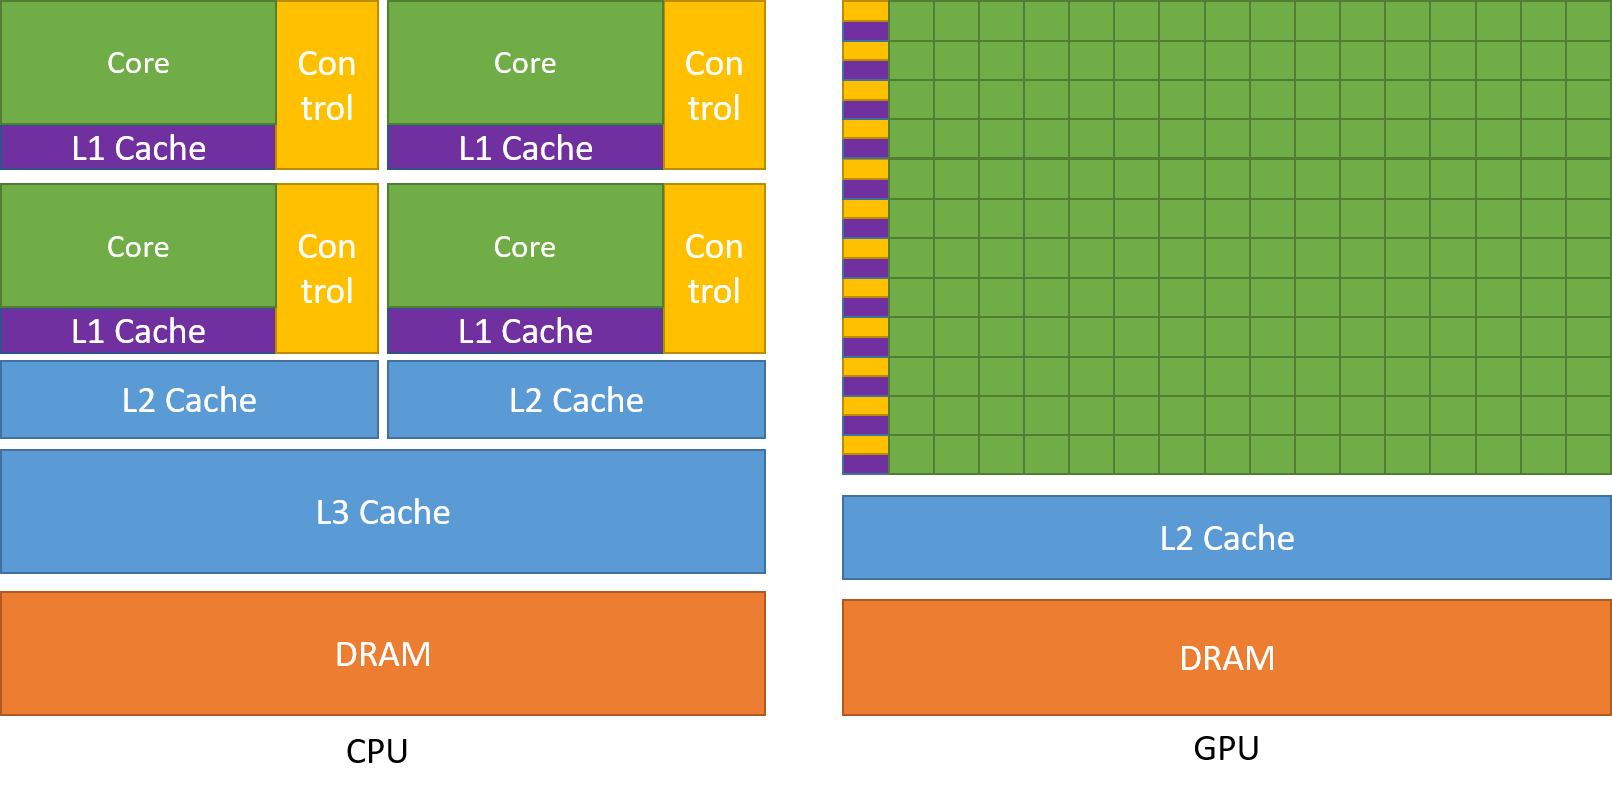
\includegraphics[width=\textwidth]{Images/gpu-devotes-more-transistors-to-data-processing.png}
        \caption{An diagram visualizing the difference between CPU and NVIDIA GPU architectures\cite{CPP_GUIDE}}
        \label{fig:enter-label}
    \end{figure}

    In this diagram, we can see that CPUs have a few number of cores and a a 3-tier cache hierarchy along with Dynamic Random Access Memory (DRAM). Each core has its own L1 Cache, going up, a few cores can share an L2 Cache, going further, all cores may access an L3 cache along with the DRAM. What the diagram does not detail is the size difference between L3 Cache and DRAM which is dramatically larger than the L3 cache, although access to the L3 cache is substantially faster than the DRAM. The diagram also omits complexity with multiple CPU cores attempting to access the large pool of memory in DRAM concurrently.

    In this same diagram, the GPU has a dramatically higher core count (green rectangles forming a grid), and cache memory is stored separate from the cores themselves, whereas the on the CPU, L1 Cache memory is stored directly near the core. While each core on the CPU may have its own control, the GPU also relegates these off the core itself. The diagram omits another facet of DRAM, and that is how the DRAM is accessed by the cores, and that all cores can access and write to this at the same time without any complex access scheduling. GPUs also maintain this DRAM separate from the system on which they are installed, allowing the card to manage memory separate from the hosting system.

    This memory management strategy is paramount to the speedups possible. As cores, despite having slower execution speed and more overhead, can perform thousands of operations at the same time, compared to the relatively few that may execute at the same time on the CPU. 
    

\section{History and Development of CUDA}
CUDA was released in 2007 by NVIDIA to provide software developers a way to utilize the unique architecture of their GPUs to accelerate the speed of scientific computations. Thanks to CUDA, GPUs have a vast number of applications beyond the rendering of graphics and into general purpose computing.

    \subsection{Origins and Milestones}
    In the eight year gap between the release of NVIDIA's GeForce 256 GPU in 1999 and the release of the CUDA programming model in 2007, there were various alternative that developers and programmers would use to utilize the properties of graphics cards, most notably the Microsoft's DirectX API, Khronos Group's OpenGL API, and NVIDIA's Cg programming language. The design of these APIs were to specifically manipulate graphical elements and shading but were also capable of performing general purpose computations\cite{CG_TUTORIAL}\cite{DIRECTX7}\cite{OPENGL1.0}. Of these, Cg set the groundwork for what would become CUDA as it provided NVIDIA a base to work with for developing an API that would allow for a more general purpose way to interact with the GPU without requiring rendering to a monitor.
    
    \subsection{Growth and Adoption in Industry}
    Long before 1999, graphics rendering had been a major role in the development of video games, and players desired more realistic graphics and more colorful video games. With the release of graphics cards, players no longer needed to purchase video game consoles which had proprietary graphics rendering modules, and could instead create computers that were capable of rendering increasingly realistic graphics.

    Outside of video games, graphics rendering was essential for data visualization applications. Receiving large data sets, and translating them to visual media has been an important role of computers. However, three dimensional data models require a large amount of processing capability, especially for models that require interaction (say rotating a three dimensional data model to get multiple perspectives).

   Film and movies had strongly relied "practical effects" to create dramatic and dynamic scenes prior to the 1970s. Complex and elaborate props and costumes were required to perform otherwise impossible feats of storytelling. Movies like the 1977 film Star Wars used highly detailed miniature sculptures of space ships as well as puppets and costumes for alien characters\cite{STAR_WARS}, a practice that had been refined by that time. But starting with the 1973 movie Westworld, computer rendering had began to enter the film industry. Until 1995, computer rendering had only been an additional aspect of film and movies, but the release of Toy Story (a move created and rendered entirely on computers) had shown that the rendering capability of computers can be used to create entire movies. Today, computer-generated imagery (CGI) has become an essential aspect of many movies and TV shows, requiring more powerful computers to render increasingly complex effects\cite{MOVIES_CGI}.

   These developments had lead to the need for increasingly powerful computers and graphical processing units. But beyond the purely graphical needs, GPUs would solve another issue, as computers would also need to take data and process it as an input, requiring a computer to not only translate two and three dimensional imagery into data points, but process them and extract meaningful data from provided imagery. Image processing would see various industry applications ranging form processing medical scans to geographical surveys. Using GPUs programmers could process data using the unique architecture of GPUs. This need to process given visual data is what would later lead to the creation of a programming model for processing multidimensional data.

\section{CUDA Programming Model}
CUDA's core strength over former GPU programming models lies in its unique compatibility with existing programming languages and its ability to cooperate with them in a fluid and understandable way familiar to those with knowledge of these languages. CUDA's Kernel Functions and Thread Hierarchy remain an intuitive part of its model, reminiscent of existing multi-threading libraries. The Memory Model and Hierarchy are at the heart of CUDA's efficiency, allowing for CRCW PRAM on Global Memory as well as a unique shared memory. And lastly, the communication and synchronization between threads and processes makes CUDA a powerful tool for programmers.

To better understand the terminology used, a GPU can be considered a "Device" due to it being external of the system which is acting as it's "Host". This "Host" is considered to be a system in which the device is installed. This system has its own CPU, memory, and storage devices that make a conventional computer system.

    \subsection{Execution Space Specifiers}
    Before breaking down the programming model, it is important to establish the concept of Execution Space Specifiers. These specifiers are integral for designating where memory and kernel functions may or may not be accessed. there are "global", "host", and "device" specifiers. A global specifier indicates that a kernel function or memory may be called or accessed by both the host and device, A host specifier will indicate strict host-only access, and a device specifier will indicate device-only access. This functionality helps differentiate what can be accessed and can help prevent errors if used correctly.

    \subsection{Kernel Functions and Thread Hierarchy}
    In order for a program to be executed in parallel, threads containing the instructions for execution must be created by the host. The instructions these threads contain are located in Kernel Functions, which are written to run exclusively on the device. While using the C++ CUDA API, these Kernel Functions behave according to the C instruction set, losing access to many of the features of C++ due to CUDA's requirement of strict memory maintenance. Because of this memory maintenance, only primitive and pointer values (to device memory only) may be passed.
    
    When creating threads from Kernel Functions, a programmer must also specify how many blocks of threads and threads per block are created to the "Grid" of blocks. The Grid is a logical structure which "contains" all thread blocks, thread blocks are a logical structure which "contain" the threads created within them. The importance behind this structure compared to a simple pool of threads is the usage of "shared" memory unique to each block of threads. A visualization of this hierarchy can be seen in Figure \ref{fig:Thread-Hierarchy}.

    \begin{figure}[!h]
        \centering
        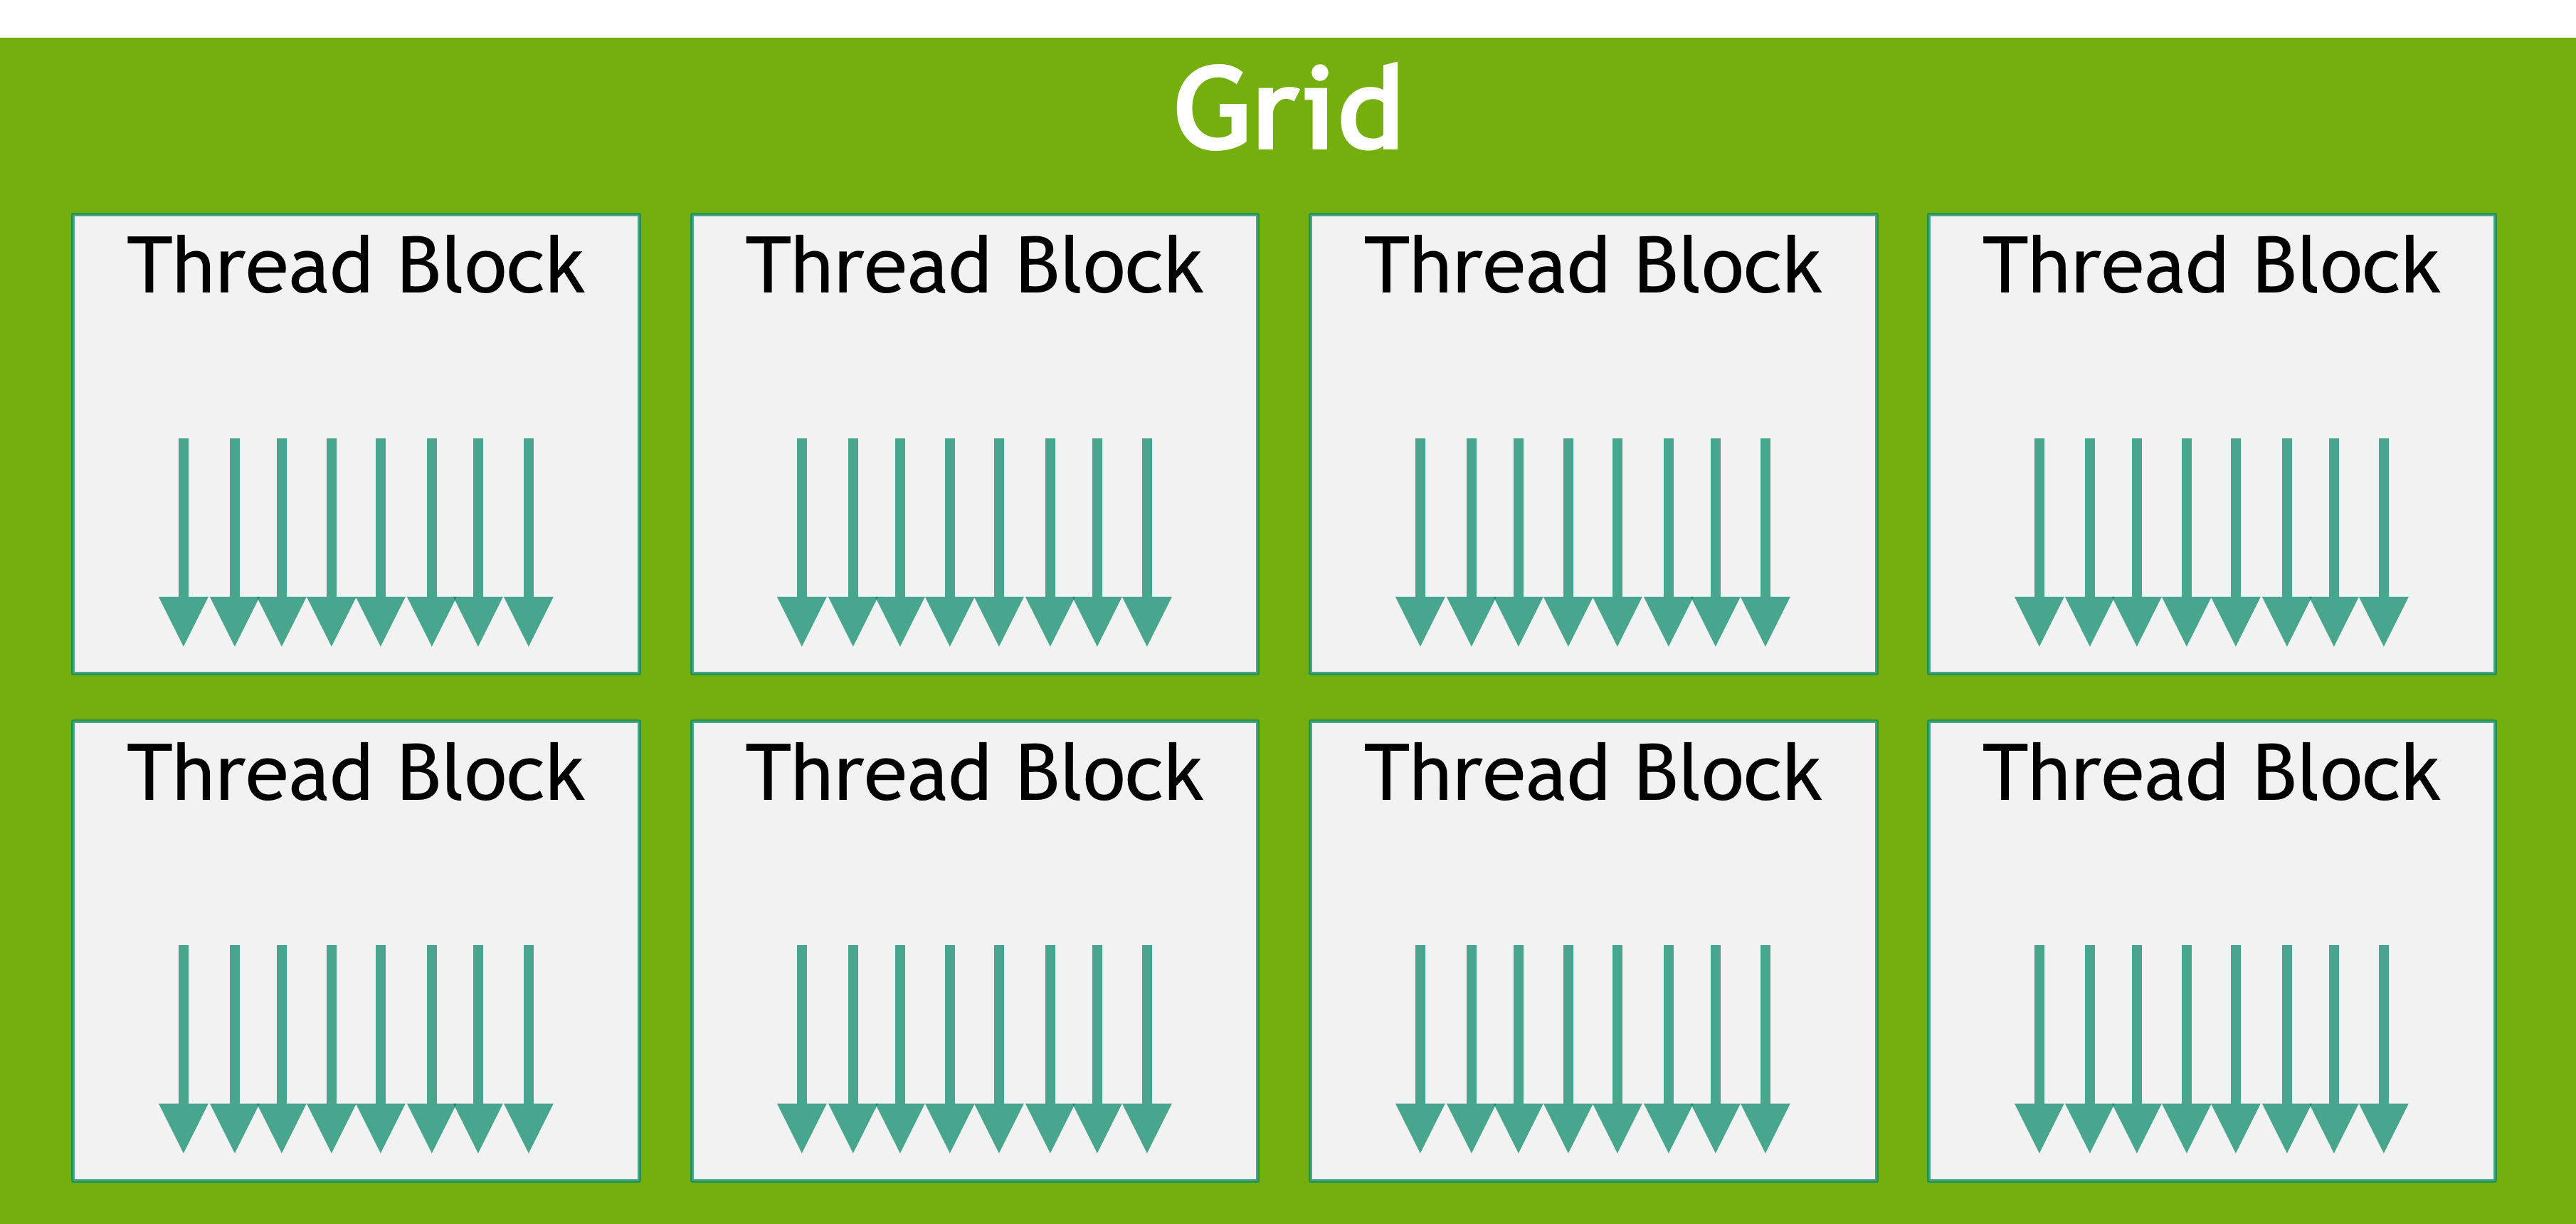
\includegraphics[width=\textwidth]{Images/grid-of-thread-blocks.png}
        \caption{Threads (visualized by green arrows pointing down) exist as part of a Thread Block, which are all contained on the Grid.\cite{CPP_GUIDE}}
        \label{fig:Thread-Hierarchy}
    \end{figure}
    
    With NVIDIA's compute capability 9.0, an additional layer of thread hierarchy was introduced called "Thread Block Clusters" which exist between the Grid and Thread Blocks as a way to organize Thread Blocks together to facilitate inter-block cooperation. To date (April 22, 20224) only one commercial grade GPU, the H100, has compute capability 9.0 and thus the only one with this additional thread hierarchy\cite{CPP_GUIDE}\cite{COMPUTE_CAPABILITY}. This additional layer of coordination can assist with the manipulation of additional dimensions of data. A visualization of this additional layer can be seen in Figure \ref{fig:Thread-Hierarchy-with-Clusters}

    \begin{figure}[!h]
        \centering
        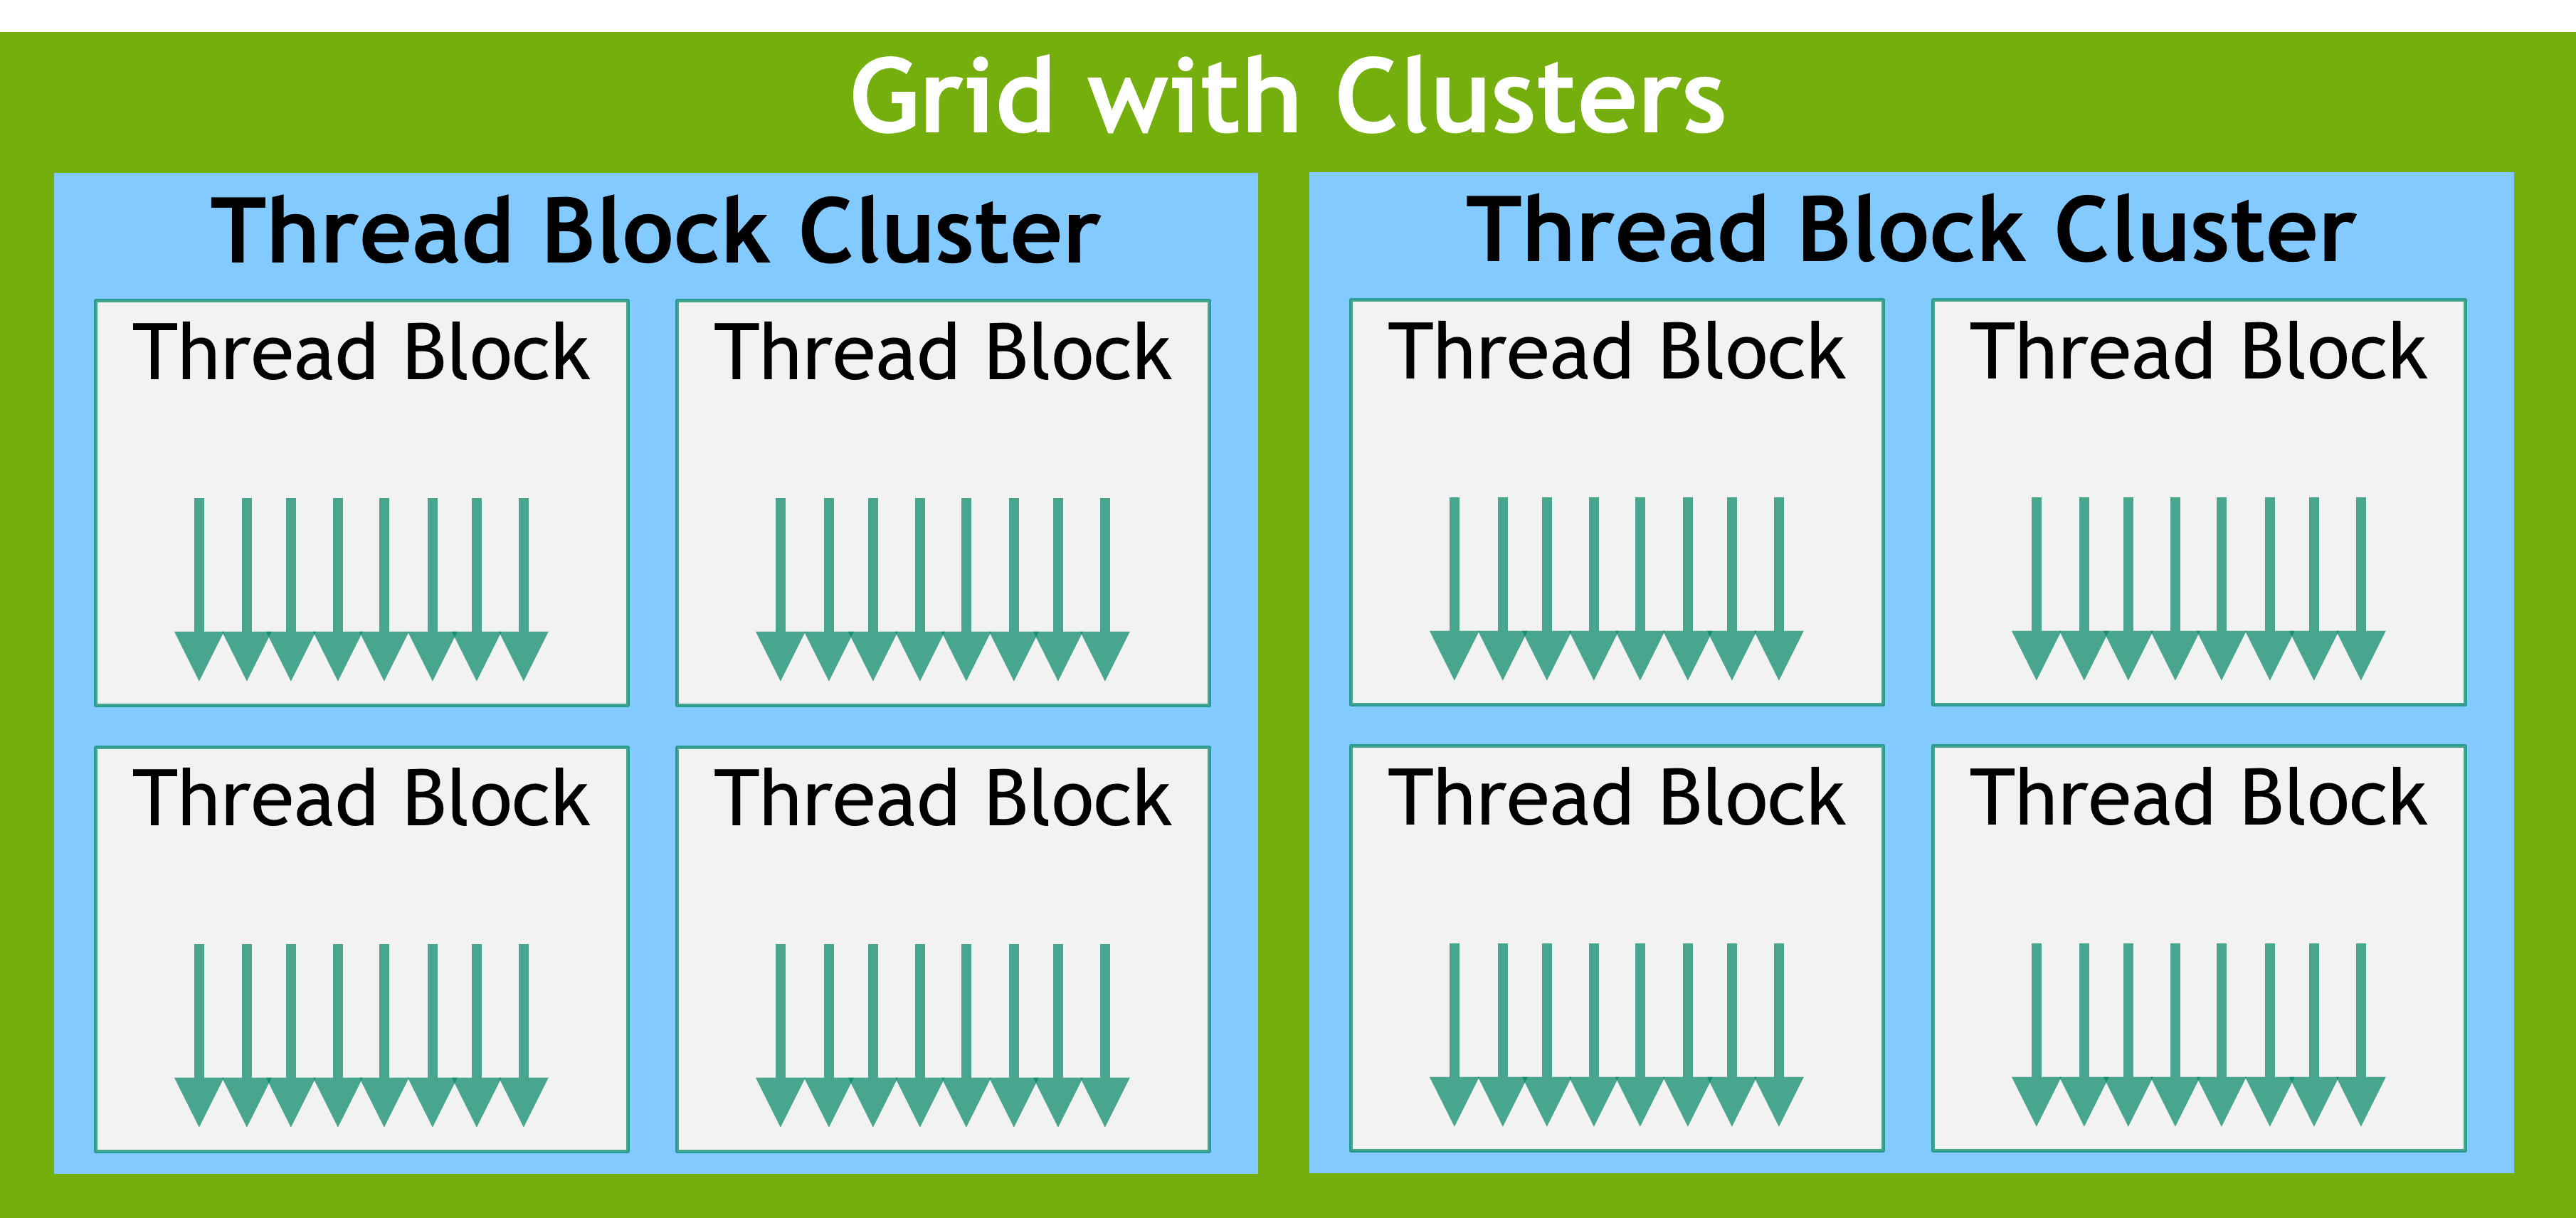
\includegraphics[width=\textwidth]{Images/grid-of-clusters.png}
        \caption{Thread Block Clusters (seen in blue) organize multiple blocks together\cite{CPP_GUIDE}.}
        \label{fig:Thread-Hierarchy-with-Clusters}
    \end{figure}
    
    \subsection{Memory Model: Global, Constant, Shared, and Local Memory}
    The CRCW structure of memory in NVIDIA GPUs is a key aspect of what makes CUDA so powerful, as conventional computing devices do not allow for thousands of threads to access and change large memory pools at the same time. But the large pool of memory is not the only structure available to threads.

    Video Random Access Memory (VRAM) is the common term for the large pool of memory available on a device; in CUDA, this is what is known as the "Global" memory. This memory is readily available for device threads to use. This memory is also available to the host, which can manipulate and copy global memory to system memory. This memory can be written to at any time by any thread running on the device, a fact which must be taken into consideration when designing Kernel functions so as to avoid overlapping read and write operations, and taking care to manage these overlaps if they must occur.

    Constant variables in memory, a feature inherent in most programming languages, is also available for writing into the global memory. Exactly who can access these variables (either host or device) can vary depending on the execution space specifier for that variable.

    As mentioned in the previous subsection, thread blocks get access to a "shared" memory which can only be accessed by threads within the same block. The device has an additional storage space specifically for this type of memory, which is inaccessible by the host, and is normally equal to the size of the global memory (though evenly distributed among the blocks existing on the grid). This shared memory is a powerful tool that allows for increased storage space in instances where process data may need to be shared between threads or process data need not be visible to the host.

    Shared memory can also exist among thread block clusters, on devices with compute capability 9.0. This distributed shared memory exists in the same space as thread block shared memory, but all threads within a thread block cluster may access memory from within the same cluster. This allows for more threads to have access to a larger shared memory space while also retaining the strengths of shared memory.

    At the thread level, each thread has access to its own local memory. The size of this local memory is relatively small compared to that which exists in shared and global memory. However, this space is sufficient for storing a large number of local variables needed for the execution of most processes. A visualization of this memory hierarchy can be seen in Figure \ref{fig:CUDA-Mem_Hierarchy}

    \begin{figure}[!h]
        \centering
        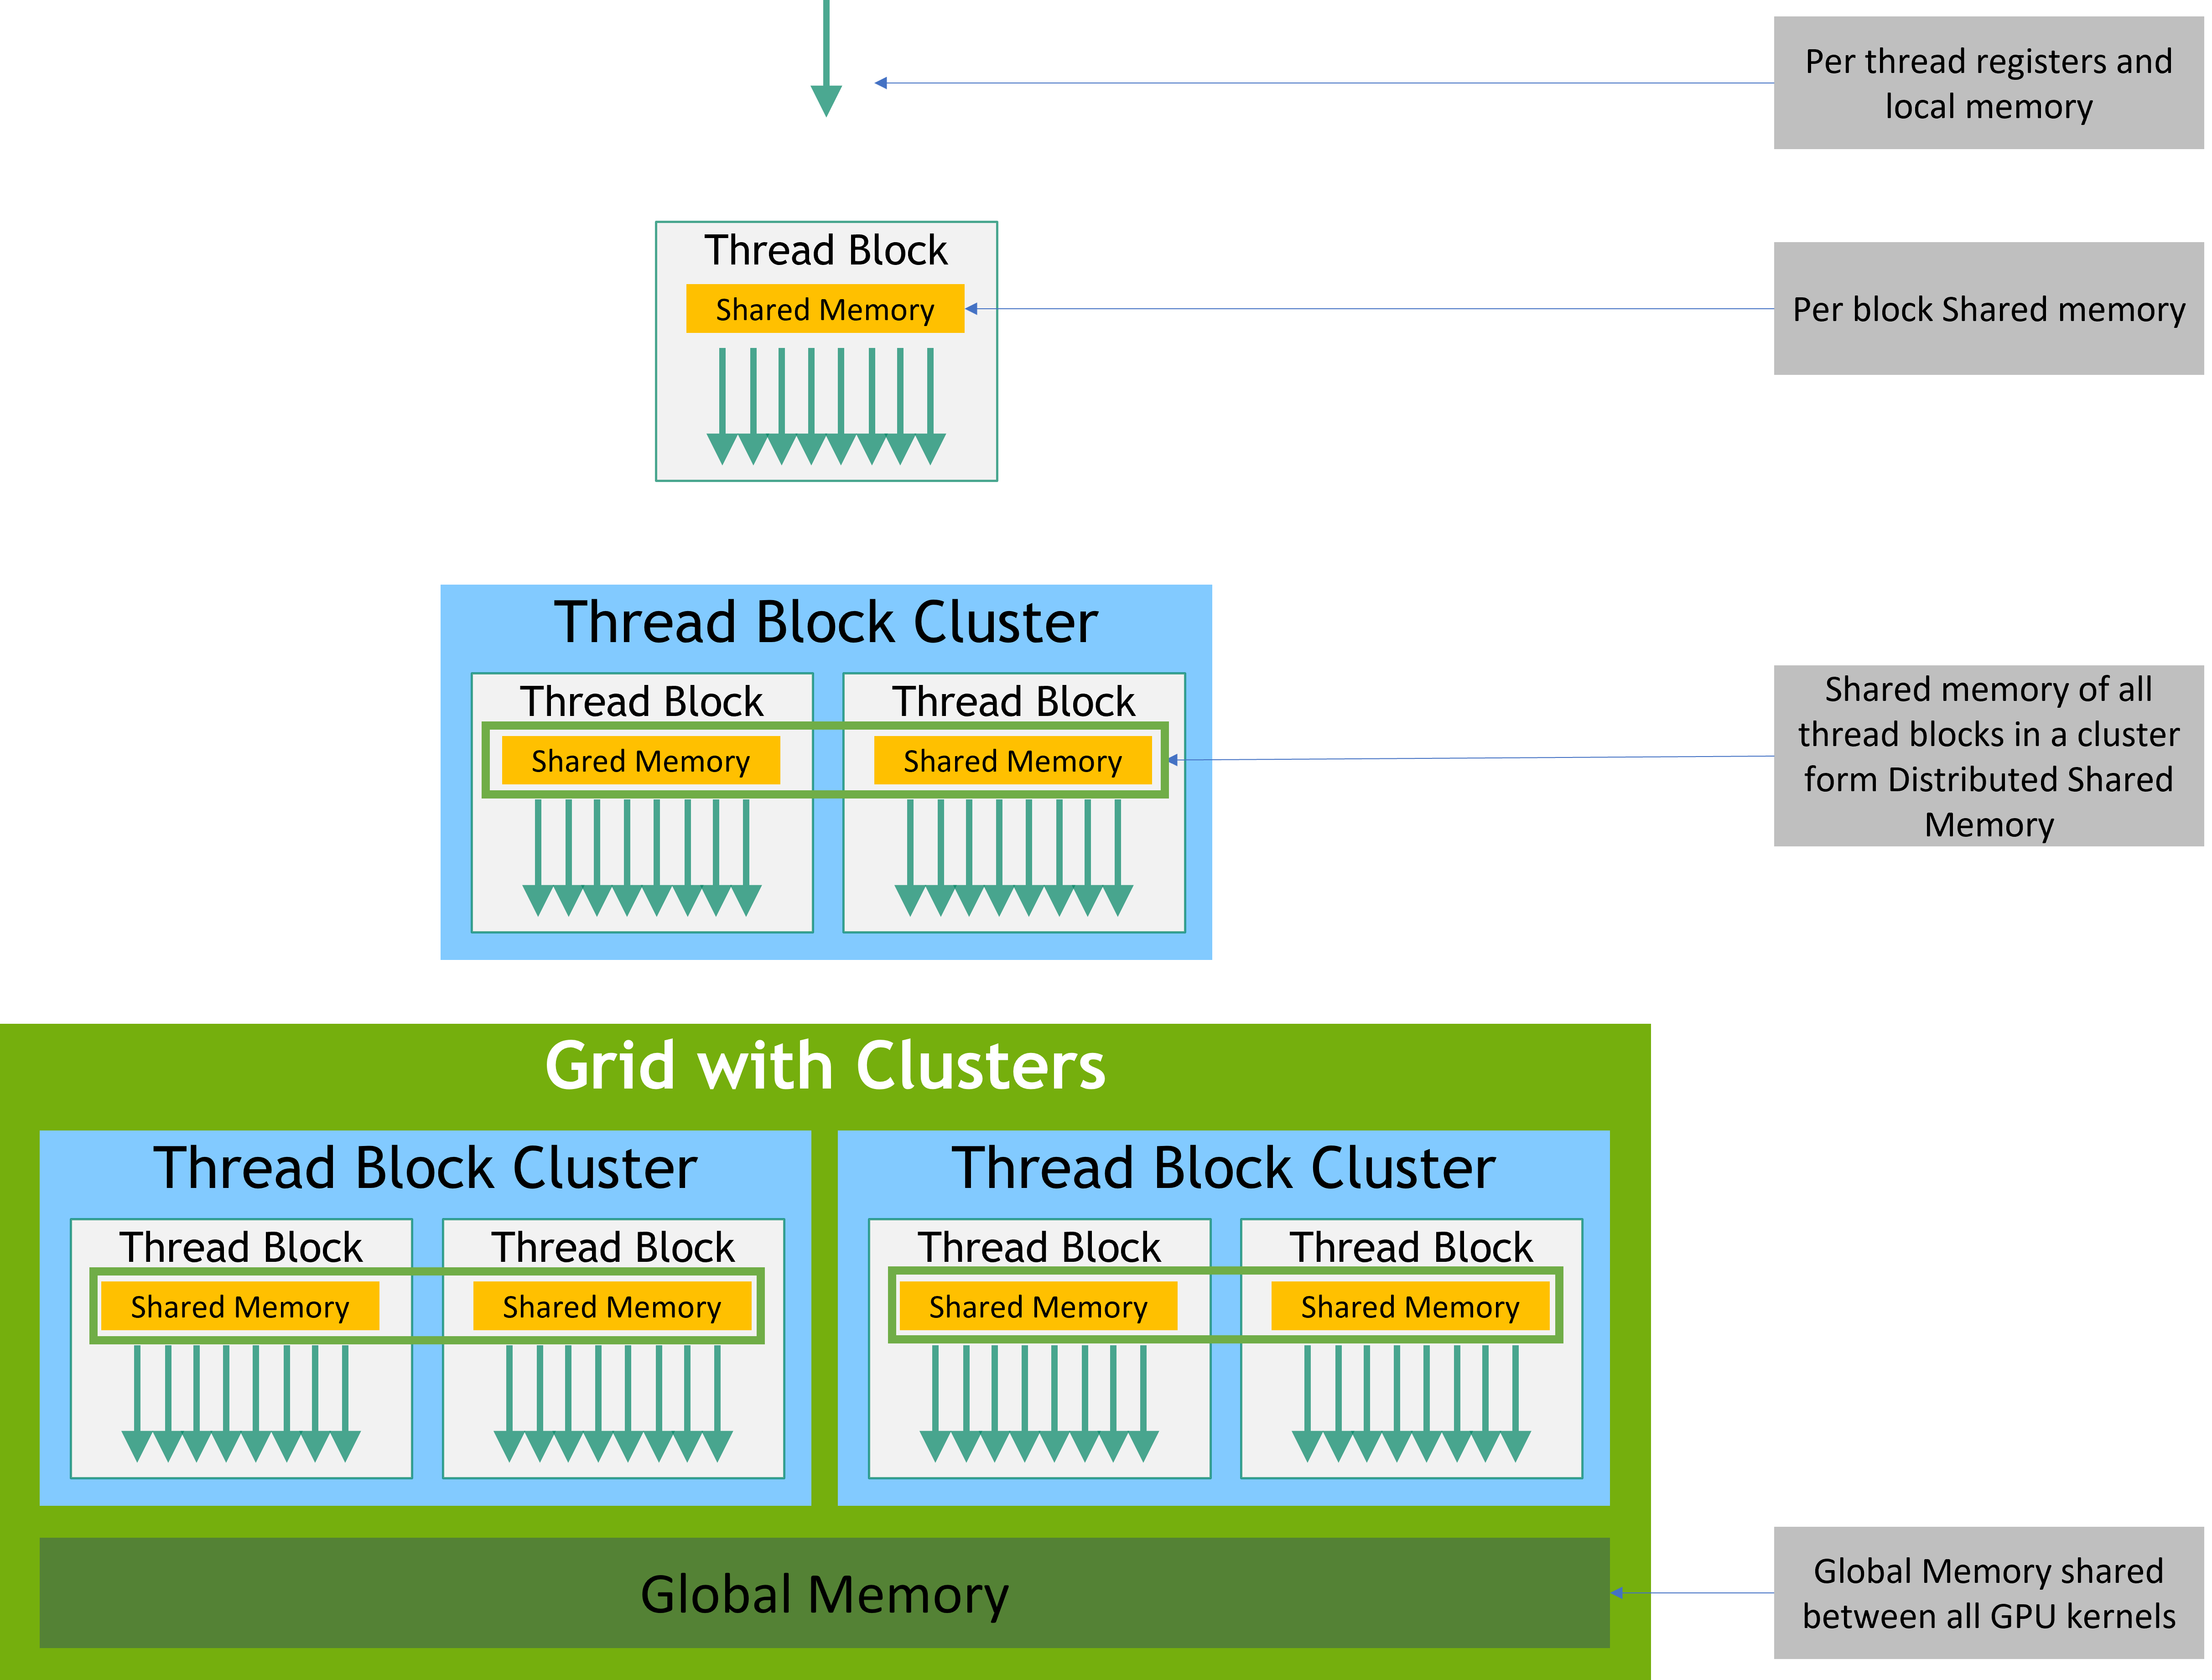
\includegraphics[width=\textwidth]{Images/memory-hierarchy.png}
        \caption{CUDA Memory Hierarchy\cite{CPP_GUIDE}.}
        \label{fig:CUDA-Mem_Hierarchy}
    \end{figure}

    

    \subsection{Synchronization and Communication}
    Before threads are created to execute on a dataset, data must first become available to these threads. The global memory is available to both the host and device which is where any data that is needed by kernel functions must be loaded. To do this, the host creates a pointer to a location in the global device memory, from which it can allocate space and copy data at that pointer. After which, upon calling a kernel function, this pointer can be passed as an argument for use by the kernel. Utilizing this functionality is key for communicating between the host and device. While kernels may alternatively access host memory, the overhead involved in directly accessing host memory from the device makes it overwhelmingly inefficient.

    In order to output data calculated on the device, the host must allocate this space before calling the kernel and pass a pointer to a location in global memory where the data is to be written. After the execution of some process on the device, the host may copy this memory to system memory. However, a problem inherent to parallel computing is how long to wait before accessing this location in memory. If it were accessed too soon, the data may not be done being written, but waiting too long may waste computation time. To resolve this, synchronization may be conducted which will force a process to wait until all threads on the device have completed. This allows the host certainty of completeness of execution. 

    Beyond this, the host process is not the only one with access to synchronization, and kernel functions may also perform synchronization. This can occur at multiple levels of the thread hierarchy, and a single thread can demand block wide synchronization, block cluster synchronization, or even grid wide synchronization. These can come in handy in instances where a thread may depend on data calculated by another thread. However, because synchronization causes a thread to wait, it can result in unnecessary idle time if used incorrectly. 

\section{Performance Optimization in CUDA}
While CUDA remains a helpful tool for parallelizing programs on a GPU, there are many ways to further improve the efficiency of the code running in parallel. Ensuring maximum GPU utilization is essential to get the most use our of a the device. Understanding memory access patters can provide significant speedups and increased memory efficiency. And the use of profiling and benchmarking tools will aid a programmer in identifying where attention should be directed in improving the efficiency of a program.

    \subsection{Techniques for Maximizing GPU Utilization}
    In most cases, maximizing utilization is directed at making sure that all cores of the device are being used at all times. To this end, it is recommended that a device be "flooded" with threads, meaning that for scalable problems, more threads are assigned to the device than there are cores available. This ensures that the maximum number of cores are being used. Ideally, flooding should occur as closely to some multiple of the number of cores that are available. For example, on an H100 GPU contains 18432 CUDA cores\cite{H100_ARCHITECTURE}, and thus to effectively flood it would mean to schedule more than that 18432 threads as close to some multiple of 18432; so an effective flood may feature 36,864 threads.

    Another technique for maximizing utilization is to ensure that the data types being used are what is required. In many situations, the data type of an 8 byte double or long offers far too much precision than the task required, and a float, int, or even short often suffice. The importance of this lies on the complexity of operations involving these data types, and large speedups can be achieved by reducing the precision of variables in use.
    
    \subsection{Understanding Memory Access Patterns}
    Due to the overhead involved in transferring memory between the host and device, keeping these operations to a minimum can substantially increase the execution speed of a program. To this end, data should only be transferred when it is absolutely required for recording purposes. In this same vein, it is also not required to allocate all memory on the host as the device. There are many data points that will only ever be used on the device, making it unnecessary for copying this data to and from the host. Addresses in memory on the device may also be re-used (provided the previous data is no longer needed), this will greatly increase the memory efficiency of a program.

    Static memory allocation (i.e. data existing in a contiguous order) should be used wherever possible, as contiguous memory access reduces time spent on the hardware searching for locations in memory. This access method also makes copying memory to and from the host a quicker process as data can be sent in one large contiguous block rather than multiple parts of the whole structure.
    
    \subsection{Profiling and Benchmarking Tools}
    A tool created by NVIDIA for profiling CUDA code is the NVIDIA Nsight Systems. It provides both a command line interface as well as a graphical user interface for creating meaningful runtime data to visualize all aspects of a program\cite{NSIGHT_USER_GUIDE}. Unlike other profiling tools, Nsight also monitors various aspects of the interaction between the host and device, so that a programmer can see how much overhead is being used during data transfers, and direct attention to further optimizing that step.

    

\section{Literature Review of CUDA Applications}
As CUDA and GPU acceleration grow in popularity, the possible speedups they provide make their use in academic research more attractive for the creation of simulations and the development of experiments involving deep learning and neural networks. 

    \subsection{Scientific Simulations and Computational Physics}
    CUDA has been used for creating environments capable of high-speed simulations that can run and calculate important data across various simulations. In a paper by Ko et. al. in 2021\cite{FLOOD_SIMULATION}, the researchers utilized CUDA to accelerate the speed at which a flood simulation was executed. The significance of their research was to produce a flood simulation to predict the damage incurred by floods in a given area.

    In an earlier simulation conducted in 2009 by Roh et. al.\cite{MOLECULAR_DOCKING}, CUDA was used to accelerate the construction and analysis of molecular stability. The implications of such research can be applied to the construction of viable drug molecules to cure and treat various diseases. This research is part of a much larger ongoing study to create software that improves on previous simulations all while using GPU-accelerated platforms like CUDA\cite{AUTODOC_MOLECULARDOCKING}.
    
    \subsection{Deep Learning and Neural Networks}
    In 2019, Rao et. al. investigated the viability of CUDA for simplifying the task of training Deep Neural Networks (DNN)\cite{ACCELERATING_DNN}. Their findings revealed that there are many steps in the training process that could be parallelized and run on a GPU. Specifically, the Backpropagation Algorithm and the Boltzmann Machine Algorithm training algorithms both feature matrix multiplication (a highly parallelizable calculation) and had that step optimized in CUDA. Using these new parallelized algorithms, the researchers observed that the elapsed time for execution was dramatically lower than the conventional implementations of these algorithms.


\section{Industrial Use Cases of CUDA}

    \subsection{Healthcare and Medical Imaging}
    In a survey conducted by Kalaiselvi et. al. in 2017\cite{CUDA_FOR_MEDICAL_IMAGING}, a multitude of applications of CUDA in medical imaging were found. Image denoising covers a wide range of approaches for providing data that doctors can use for making accurate diagnosis. One approach is adaptive filtering; with this approach, researchers compared special filtering and Fast Fourier Transform (FFT) based filtering by using a GPU implementation in CUDA and a multi threaded CPU implementation for each\cite{IMAGE_DENOISING}. Using these tests, the researchers observed massive speedups from a few days and 50 minutes using the CPU approach to 25 minutes and 8 minutes for their CUDA approach. 

    Beyond filtering, Kalaiselvi et. al. also investigated Registration (the spatial alignment between a reference image and a spatialy transformed image). One such approach is the rigid transformation estimation. Using which, researchers found substantial speedups from 7 minutes to 7 seconds when comparing a multi threaded version of the algorithm compared to one running on a GPU respectively\cite{EM_ICP_ON_GPU}.

    Another important facet of medical imaging that Kalaiselvi et. al. found that has been accelerated using CUDA is segmentation. In Kalaiselvi et. al.'s own research, they observed speedups approaching 46 times faster using CUDA than a conventional single thread approach\cite{CPU_AND_GPU_ACCELERATING_IMAGE_APPLICATIONS}.

    The last use case of medical image processing involving CUDA investigated by Kalaiselvi et. al. was visualization, the creation of easy to interpret visual media using data processed from medical images. CUDA provides a toolkit to implement software for surface rendering and volume rendering to help with the projection of data into 2-dimensional and 3-dimensional models for doctors to analyze and diagnose from.

    The implications of these advances involve faster access to accurate medical data to allow doctors to more quickly and accurately diagnose diseases in patients. As well as the creation of advanced medical imaging machinery and software for distribution to hospitals.
    
    \subsection{Logistics Optimization}
    Introduced in 2021, NVIDIA released the cuOpt API for solving optimization problems such as the Traveling Salesman Problem (TSP), the Vehicle Routing Problem (VRP), and the Pickup and Delivery Problem (PDP)\cite{WORLD_RECORD_OPTIMIZATION}\cite{CUOPT_USER_GUIDE}. This optimization API, which is powered by NVIDIA GPUs running on CUDA, has applications across various logistics and scheduling fields as it provides a way to define constraints and problem specifications on the user-end, so a multitude of problems can be solved rapidly. The exact details of cuOpt's algorithm is not readily accessible to the public due to competing interests from other competing firms, but NVIDIA does not hide the fact that it is running on servers powered by their GPUs.


\chapter{Combinatorial Optimization and Parallel Algorithms}
The exploration of combinatorial optimization problems reflects a longstanding pursuit of efficient and scalable solutions across various disciplines. Traditional sequential algorithms, though effective for smaller problem sizes, encounter limitations when confronted with large-scale combinatorial challenges. This limitation has sparked interest in leveraging parallel computing paradigms to tackle optimization tasks more effectively.

Chapter 2 will delve into the landscape of parallel optimization algorithms, highlighting the evolution from classical sequential approaches to sophisticated parallel strategies. As the focus shifts to Section 2.1, an insightful overview of combinatorial optimization problems is presented—ranging from well-known conundrums like the Traveling Salesman Problem to graph-based challenges like graph coloring and maximum clique.

This section aims to establish a foundational understanding of the diverse problem spaces within combinatorial optimization, setting the stage for subsequent discussions on parallel algorithm design and GPU-accelerated solutions. By contextualizing these problems, the report paves the way for exploring how the CUDA architecture can be harnessed to address these challenges efficiently and at scale.

    \section{Overview of Combinatorial Optimization Problems}
    Combinatorial optimization problems encompass a diverse range of challenges that involve making optimal selections or decisions from a finite set of discrete possibilities\cite{papadimitriou1998combinatorial}. These problems are often characterized by discrete decision variables and non-linear objective functions, making them computationally complex to solve\cite{korte2011combinatorial}. The solutions to combinatorial optimization problems are crucial in addressing real-world problems across multiple domains. 
        \subsection{Types of Combinatorial Problems}

        \subsubsection{Traveling Salesman Problem (TSP)}
        The Traveling Salesman Problem (TSP) stands as one of the most extensively studied combinatorial optimization problems in computer science, logistics, and operations research. This classic algorithmic problem serves as a standard benchmark for evaluating the efficacy of various combinatorial algorithms due to its complexity and practical applications.

        In the TSP, a salesman is tasked with visiting a set of cities and determining the shortest possible route that allows him to visit each city exactly once and return to his original location. Despite its seemingly simple problem statement, the TSP is classified as an NP-hard problem in combinatorial optimization, representing a significant challenge in both operations research and theoretical computer science.

        \begin{figure}[h!]
            \centering
            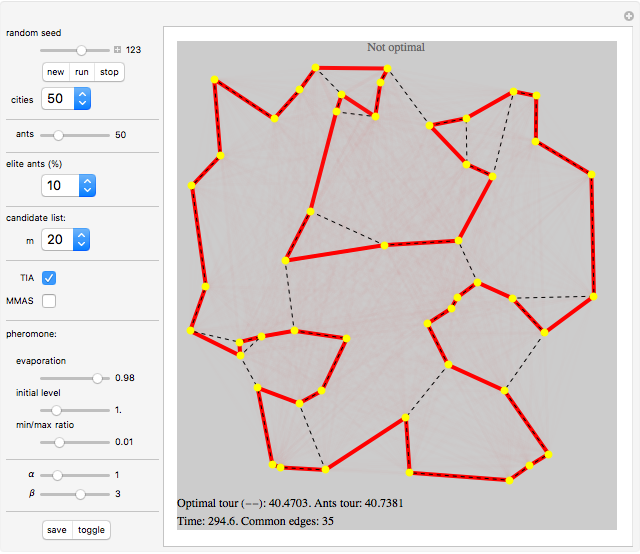
\includegraphics[width=0.75\textwidth,keepaspectratio]{Images/aco_tsp.png}
            \caption{A graphical representation of solutions for the Traveling Salesman Problem. The global optimum is represented by a dashed line, and the current found solution is the solid red line. This picture showcases a simulation of Ant Colony Optimization, discussed later in this chapter.}
            \label{fig:aco-demo}
        \end{figure}
        
        Mathematically, if there are $n$ cities, the number of possible routes to consider grows factorially as $n!$, rendering exact solutions computationally infeasible for large instances. This exponential growth in the solution space underscores the difficulty of finding an optimal solution using traditional methods. As a result, researchers have developed heuristic and metaheuristic approaches to approximate optimal or near-optimal solutions within reasonable computation time.
        
        Heuristic methods for solving the TSP include algorithms like nearest neighbor, genetic algorithms, simulated annealing, and ant colony optimization. These approaches sacrifice optimality for computational efficiency, leveraging iterative improvement techniques to converge towards a good solution within acceptable time limits.
        
        The TSP and its variants find widespread applications in logistics, transportation planning, network design, and manufacturing. For instance, in logistics and delivery services, optimizing delivery routes using TSP-based algorithms can minimize travel costs and reduce delivery times. Similarly, in network design, the TSP is used to optimize data routing and minimize latency in communication networks.
        
        The continuous research and development efforts dedicated to solving the TSP highlight its significance as a fundamental problem in combinatorial optimization, with implications across various industries and scientific disciplines. The quest for efficient solutions to the TSP continues to drive innovation in algorithm design and computational optimization techniques.

        \subsubsection{Knapsack Problem}
        The Knapsack Problem is a classic optimization problem that involves selecting a subset of items to maximize value or utility while respecting a given weight or capacity constraint\cite{CACCHIANI2022105693}. The problem can be categorized into two main variants: the 0/1 Knapsack Problem and the Fractional Knapsack Problem.

        \begin{itemize}
            \item 0/1 Knapsack Problem: In this variant, each item can either be included in the knapsack (represented by a binary decision) or excluded. The objective is to determine the optimal combination of items that maximizes the total value without exceeding the knapsack's weight capacity. The 0/1 Knapsack Problem is NP-hard, meaning that there is no known polynomial-time algorithm that guarantees an optimal solution for all instances.

           \item Fractional Knapsack Problem: Unlike the 0/1 Knapsack Problem, the Fractional Knapsack Problem allows items to be divided into fractions. Each item has a weight and a corresponding value, and the goal is to select fractions of items to maximize the total value without exceeding the knapsack's weight capacity. The Fractional Knapsack Problem can be solved using a greedy algorithm, where items are selected based on their value-to-weight ratio until the knapsack is full.
        \end{itemize}

        \begin{figure}[h!]
            \centering
            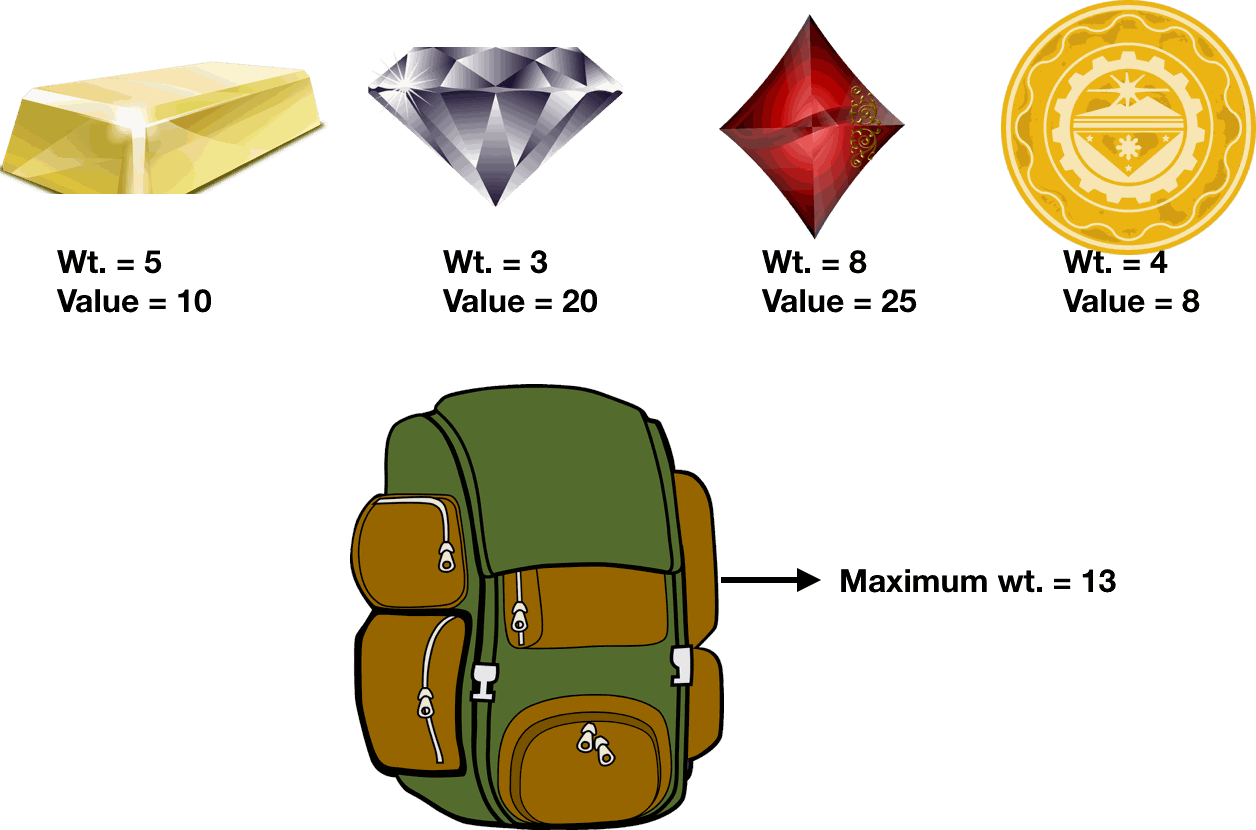
\includegraphics[width=0.75\textwidth,keepaspectratio]{Images/knap1.png}
            \caption{A basic representation of the Knapsack Problem. The backpack can hold at most 13, and figuring out how to pack the backpack in such a way that the value is maximized is not immediately intuitive.}
            \label{fig:knap-demo}
        \end{figure}

        Applications of the Knapsack Problem extend to various domains, including resource allocation, project scheduling, and financial portfolio optimization. For instance, in resource allocation scenarios, the Knapsack Problem can be used to optimize inventory management by selecting the most valuable items within capacity constraints. Similarly, in portfolio optimization, investors aim to maximize returns while adhering to constraints on risk exposure and investment limits, akin to the Knapsack Problem's constraints on weight capacity.
        
        The Knapsack Problem illustrates the trade-off between maximizing utility and respecting resource limitations, making it a fundamental problem in combinatorial optimization. Its computational complexity and practical applications underline its significance in decision-making and resource allocation strategies across industries.

        \subsubsection{Graph Coloring Problem}
        Graph coloring algorithms are essential tools for optimizing resource usage and minimizing interference in various network design applications. The Graph Coloring Problem, which entails assigning colors to the vertices of a graph such that no two adjacent vertices share the same color, has broad applications across diverse disciplines\cite{jensen2011graph}. 

        \begin{figure}[h!]
            \centering
            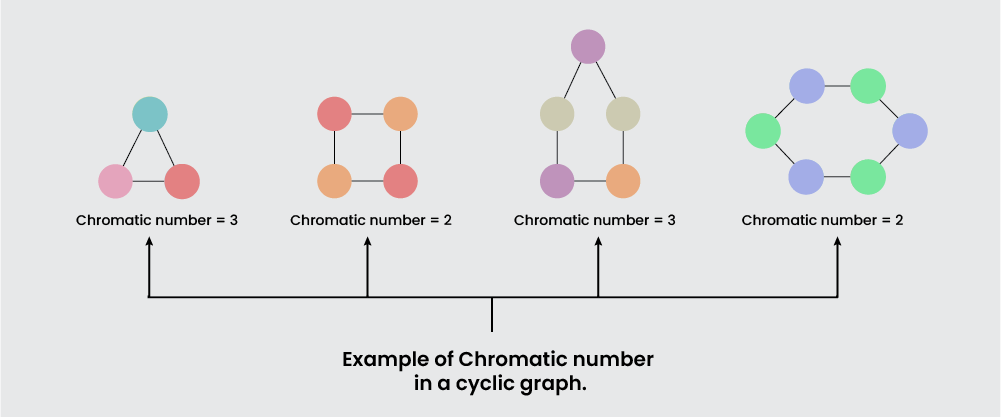
\includegraphics[width=0.75\textwidth,keepaspectratio]{Images/chromatic-number-of-cycle-graph-example.png}
            \caption{The minimum number of colors needed to color a graph is called its chromatic number. This figure demonstrates various graphs of chromatic number 2 and 3.}
            \label{fig:chromatic_number}
        \end{figure}

        One key area where graph coloring algorithms find application is in register allocation within compilers. In computer science, compilers translate high-level programming languages into machine code. Efficient register allocation is critical for optimizing program performance by minimizing memory access and maximizing CPU utilization. Graph coloring techniques are employed to assign processor registers to variables, ensuring that no two variables that are simultaneously active share the same register.
        
        Another important application of graph coloring is in frequency assignment for wireless communication networks. In wireless networks, assigning frequencies to communication channels is crucial to minimize interference and optimize signal quality. By representing network topology as a graph and applying graph coloring algorithms, wireless network engineers can efficiently allocate frequencies to different communication channels, thereby improving overall network performance and reliability.
        
        Moreover, graph coloring algorithms have implications in scheduling problems across various industries. For instance, in project management, scheduling tasks with resource constraints can be modeled as a graph coloring problem. Each task represents a vertex, and resource constraints (e.g., availability of equipment or personnel) translate into constraints on the colors assigned to vertices.
        
        Graphs are ubiquitous mathematical structures used to represent relationships and interconnections in diverse contexts, ranging from social networks and transportation networks to biological networks and resource allocation problems. By leveraging graph coloring algorithms, researchers and practitioners can tackle complex optimization challenges and derive efficient solutions in real-world applications across multiple domains.

        \subsubsection{Maximum Clique Problem}
        The Maximum Clique Problem is a fundamental problem in graph theory that involves identifying the largest subset of vertices in a graph such that every pair of vertices in the subset is connected by an edge. In other words, the goal is to find a clique (a subset of vertices where every pair of vertices is adjacent) that is as large as possible.

        The problem is NP-hard, meaning that finding the maximum clique in a graph is computationally challenging, especially for large graphs. Due to its complexity, the Maximum Clique Problem has applications in various fields, including social network analysis, bioinformatics, and graph-based community detection.
        
        In social network analysis, identifying maximum cliques helps reveal cohesive groups or communities within a network, shedding light on patterns of connectivity and interaction among individuals or entities. In bioinformatics, maximum cliques are used to analyze protein interaction networks and genetic networks, providing insights into functional relationships among biological entities.

        \begin{figure}[h!]
            \centering
            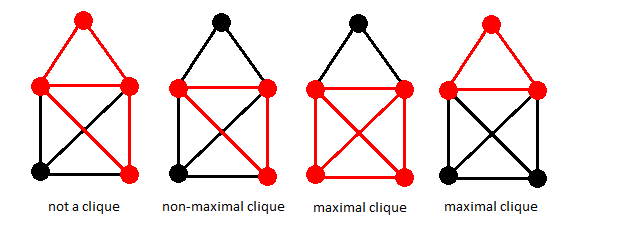
\includegraphics[width=0.75\textwidth,keepaspectratio]{Images/clique.png}
            \caption{A simple 5 node graph with vertex connections showing different clique behaviors based off of the completeness of the connections.}
            \label{fig:clique-demo}
        \end{figure}
        
        Efficient algorithms for finding maximum cliques include branch-and-bound techniques, heuristic methods based on graph coloring and backtracking, as well as advanced optimization approaches leveraging mathematical programming formulations.

        \subsubsection{Integer Linear Programming (ILP)}
        Integer Linear Programming (ILP) is a mathematical optimization technique that involves optimizing a linear objective function subject to linear inequality and equality constraints, with the additional constraint that decision variables must take integer values. ILP is a powerful tool for modeling and solving a wide range of combinatorial optimization problems.

        \begin{figure}[h!]
            \centering
            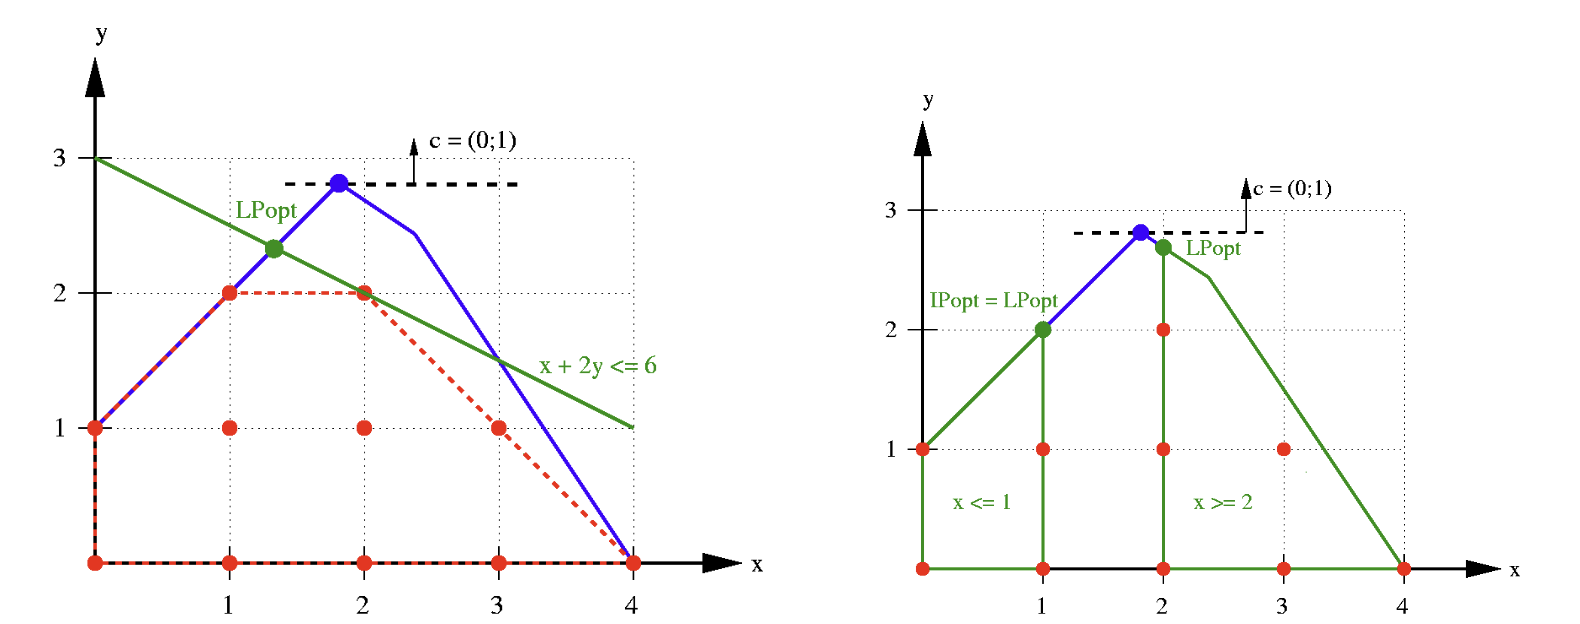
\includegraphics[width=0.9\textwidth,keepaspectratio]{Images/integer-linear.png}
            \caption{A convex linear integer programming problem showing multiple competing constraints creating a boundary for the search space. The optimal value in a convex ILP problem is always on one of the vertices of the solution space.}
            \label{fig:ilp-demo}
        \end{figure}

        In ILP, decision variables are represented as integers, allowing for the formulation of complex optimization problems involving discrete choices. ILP finds applications in resource allocation, production planning, scheduling, and logistics optimization across industries.
        
        For example, in production planning, ILP is used to optimize production schedules by determining the optimal allocation of resources (e.g., machines, labor) to meet demand while minimizing costs and fulfilling capacity constraints. Similarly, in supply chain management, ILP is employed for inventory optimization, distribution planning, and transportation logistics.
        
        ILP problems are solved using specialized algorithms such as branch-and-bound, cutting-plane methods, and advanced linear programming solvers. The ability to model discrete decision variables makes ILP a versatile and widely applicable optimization framework for addressing complex real-world problems efficiently.

        \subsubsection{Pickup and Delivery Problem (PDP)}

        The Pickup and Delivery Problem (PDP) is a combinatorial optimization problem that involves coordinating the movement of goods or resources between locations, where each location has both a pickup and a delivery requirement. The objective of the PDP is to determine an optimal sequence of pickups and deliveries that minimizes transportation costs, travel time, or other specified objectives, subject to various constraints.
        
        In the PDP, a set of pickup requests and corresponding delivery requests must be fulfilled using a limited fleet of vehicles or transport units. Each request specifies the quantity and type of goods to be picked up at a given location and delivered to another location. The challenge lies in efficiently assigning vehicles to pickup and deliver tasks while optimizing route plans to maximize resource utilization and minimize operational costs.
        
        The Pickup and Delivery Problem is a generalization of traditional vehicle routing problems (VRPs) and encompasses additional complexities associated with pickup and delivery operations. Key characteristics of the PDP include:

        \begin{itemize}
            \item \textbf{Constraints:} Various constraints may apply, such as vehicle capacities, time windows for pickups and deliveries, compatibility constraints between pickup and delivery tasks, and vehicle availability.
        
            \item \textbf{Objective Function:} The goal is typically to minimize total transportation costs, travel time, vehicle usage, or a combination of these factors, while satisfying all pickup and delivery requirements.
        \end{itemize}
        
        The PDP finds applications in logistics, transportation planning, supply chain management, and urban delivery services. For example, in urban freight logistics, companies must optimize the movement of goods to and from distribution centers, warehouses, and retail locations while adhering to delivery time windows and minimizing traffic congestion.
        
        Similar to other combinatorial optimization problems, the PDP is NP-hard, meaning that finding an optimal solution for large instances is computationally challenging. As a result, heuristic and metaheuristic approaches are often employed to generate near-optimal solutions efficiently.
        
        Efficiently solving the Pickup and Delivery Problem requires the development of advanced algorithms and optimization techniques that balance complex routing decisions with operational constraints. The ability to optimize pickup and delivery sequences can lead to significant cost savings, improved resource allocation, and enhanced efficiency in transportation and logistics operations.

        \subsection{Importance in Decision Making and Resource Allocation}
        Combinatorial optimization problems hold significant importance in decision-making processes and resource allocation strategies across industries due to their ability to address complex operational challenges efficiently. Optimization algorithms can be leveraged by organizations to make informed decisions that optimize resource utilization, minimize costs, and improve overall performance. One key aspect of combinatorial optimization is its role in optimal resource allocation. For instance, in logistics and transportation, solving vehicle routing problems (VRPs) ensures efficient allocation of vehicles and drivers to minimize transportation costs and meet customer service requirements. Similarly, in production planning, optimizing machine scheduling and inventory management using combinatorial optimization techniques leads to improved utilization of manufacturing resources and reduced production costs.

        Decision support systems heavily rely on solutions derived from combinatorial optimization problems to assist in strategic decision-making. These systems integrate optimization algorithms to analyze complex scenarios and recommend optimal courses of action based on predefined objectives and constraints. For example, in finance, portfolio optimization models leverage combinatorial algorithms to allocate investment assets across various financial instruments, balancing risk and return to achieve desired investment objectives. In healthcare, optimization models aid in hospital resource allocation and staff scheduling to optimize patient care delivery and operational efficiency.
        
        The impact of combinatorial optimization extends to cost reduction and operational efficiency across various sectors. By optimizing processes such as routing, scheduling, and inventory management, organizations can achieve significant cost savings and streamline operations. For instance, in retail and e-commerce, optimizing order fulfillment processes through warehouse layout optimization and order picking strategies reduces shipping costs and improves delivery speed. Similarly, in telecommunications, network optimization algorithms ensure efficient utilization of network resources, enhancing service quality and reducing operational expenses.
        
        Furthermore, the strategic planning and performance improvement facilitated by combinatorial optimization solutions enable organizations to adapt to dynamic market conditions and achieve competitive advantage. By leveraging optimization outcomes, businesses can develop data-driven strategies to optimize supply chain operations, enhance customer service, and drive business growth. The effective utilization of combinatorial optimization techniques allows organizations to make informed decisions that optimize resource allocation, improve operational efficiency, and gain a strategic edge in competitive markets.


    \section{Classical Optimization Algorithms}

    Classical optimization algorithms form the foundational basis of solving optimization problems across various disciplines, ranging from computer science and operations research to engineering and economics. These algorithms are characterized by their systematic approach to finding optimal solutions or approximations to complex optimization problems.

    The primary objective of classical optimization algorithms is to maximize or minimize an objective function subject to specified constraints, often involving discrete or continuous decision variables. These algorithms are essential tools for addressing combinatorial optimization problems, linear and nonlinear programming, and global optimization challenges.
    
    Key characteristics of classical optimization algorithms include:
    \begin{itemize}
        \item \textbf{Problem Modeling:} Classical algorithms begin by modeling the optimization problem with defined objectives, decision variables, constraints, and optimization criteria. This process involves transforming real-world problems into mathematical formulations that can be solved algorithmically.
    
        \item \textbf{Optimization Techniques:} Classical algorithms employ a range of techniques, including exact methods such as dynamic programming and branch-and-bound, as well as heuristic methods such as greedy algorithms and genetic algorithms, to explore and navigate the solution space efficiently.
    
        \item \textbf{Performance Evaluation:} Evaluating the performance of classical optimization algorithms involves analyzing their convergence properties, computational complexity, scalability, and solution quality. Comparative studies help identify the most suitable algorithmic approach for specific optimization problems.
    \end{itemize}
    
    Classical optimization algorithms are covered in this section, beginning with an overview of greedy algorithms followed by discussions on other fundamental techniques such as dynamic programming, branch-and-bound, and metaheuristic approaches. Understanding these algorithms provides a comprehensive foundation for tackling optimization challenges and developing efficient solutions across diverse application domains.

        \subsection{Greedy Algorithms}
        A greedy algorithm is a simple yet powerful approach used to solve optimization problems by making locally optimal choices at each step. The strategy involves selecting the best available option in the current iteration without considering future consequences, aiming to achieve immediate optimization. While often intuitive and efficient, greedy algorithms may not always yield globally optimal solutions due to their myopic decision-making process.

        An example of the greedy approach applied to the TSP is provided, and the strengths and weaknesses of this approach are clearly relevant and consistent among other optimization problems\cite{GUTIN200281}.

        In the context of the TSP, a natural and intuitive greedy strategy is the nearest neighbor algorithm (NN). This approach involves starting from an arbitrary city and repeatedly selecting the closest unvisited city as the next destination. This process continues until all cities are visited; the process of visiting all cities and returning to the arbitrary starting location forms the tour. 

        \begin{figure}[h!]
            \centering
            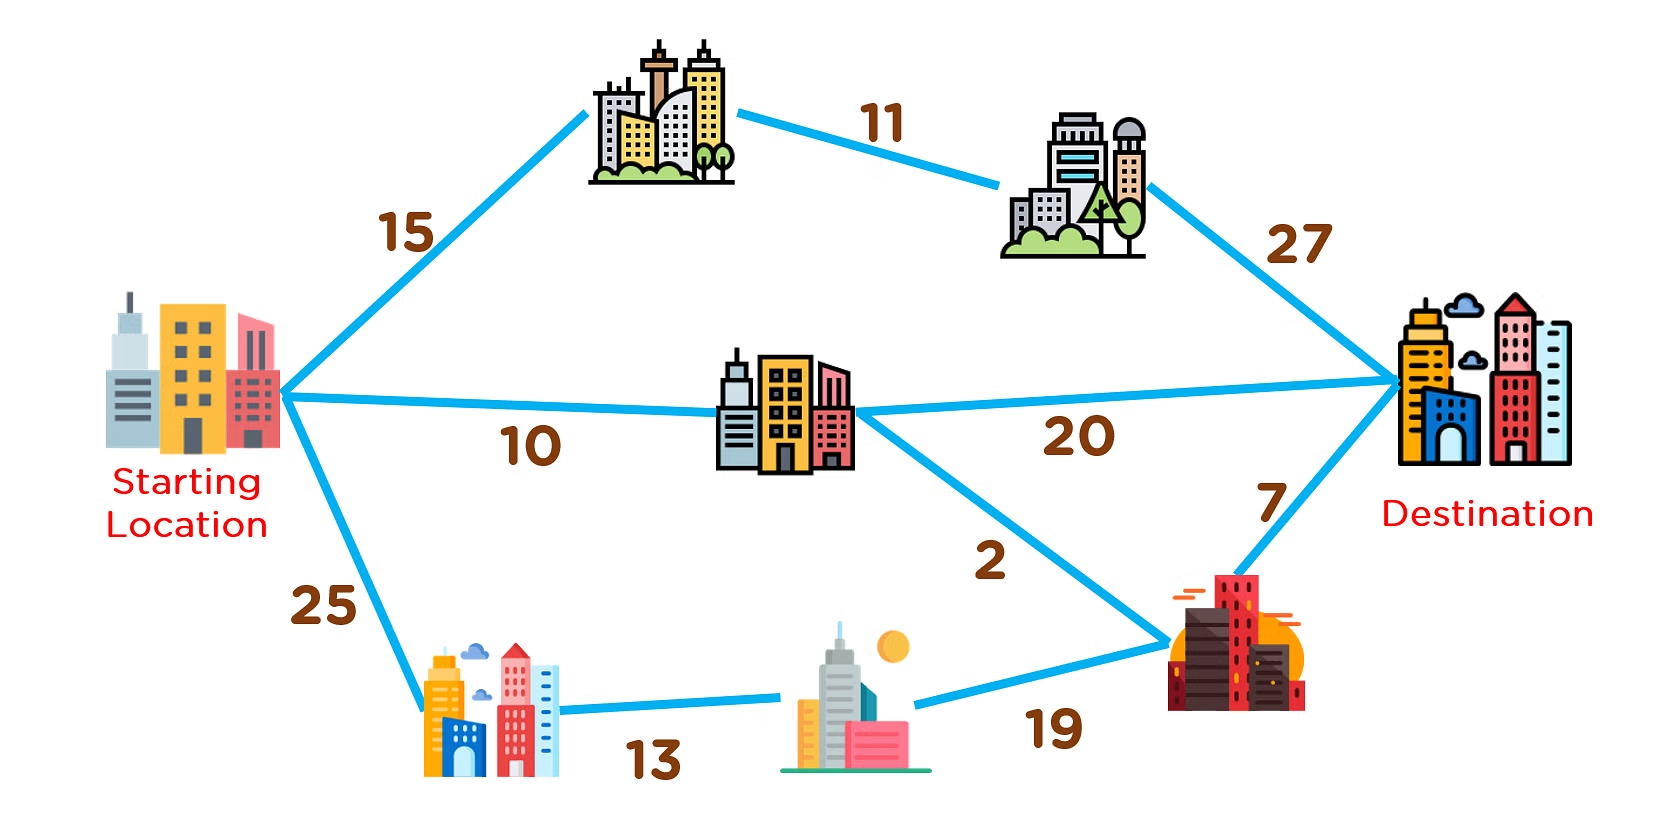
\includegraphics[width=0.9\textwidth,keepaspectratio]{Images/Thumbnail_Greedy_Problem.jpg}
            \caption{A simple pathfinding problem where the greedy solution produces the shortest route from start to destination by repeatedly selecting the edge with the smallest weight from the current city.}
            \label{fig:greedy-tsp-good}
        \end{figure}

        The nearest neighbor algorithm is straightforward and computationally efficient, making it an appealing choice for solving the TSP\cite{reinelt2003traveling}. However, despite its simplicity, this greedy approach does not guarantee finding the optimal tour due to its myopic decision-making.

        Research has demonstrated that the nearest-neighbor greedy approach for the TSP can produce suboptimal tours\cite{cirasella2001asymmetric}, and in fact, may lead to the unique worst possible tour in certain scenarios\cite{gutin2005evaluation}. The key limitations arise from the algorithm's inability to consider the global structure of the problem and optimize across all cities simultaneously\cite{GUTIN200281}. Suppose, in a different problem, a person was faced with a decision to either go down a path leading to the left or a path leading to the right. On the left path in front of them is a large sum of money, but nothing else the entire path. On the right path, there is nothing visible, but a large sum of money waits on each milemarker of the path. The person in this example is using the greedy approach, and opts to select the left path. However, unbeknownst to the person at the time, the right path has a much larger sum of money by the end of the trail. The person, using the greedy approach, didn't consider that their short term optimal decision might not end up being the long term best decision. This example is very rudimentary, but highlights the short term decision making involved in using a greedy algorithm.  

        \begin{figure}[h!]
            \centering
            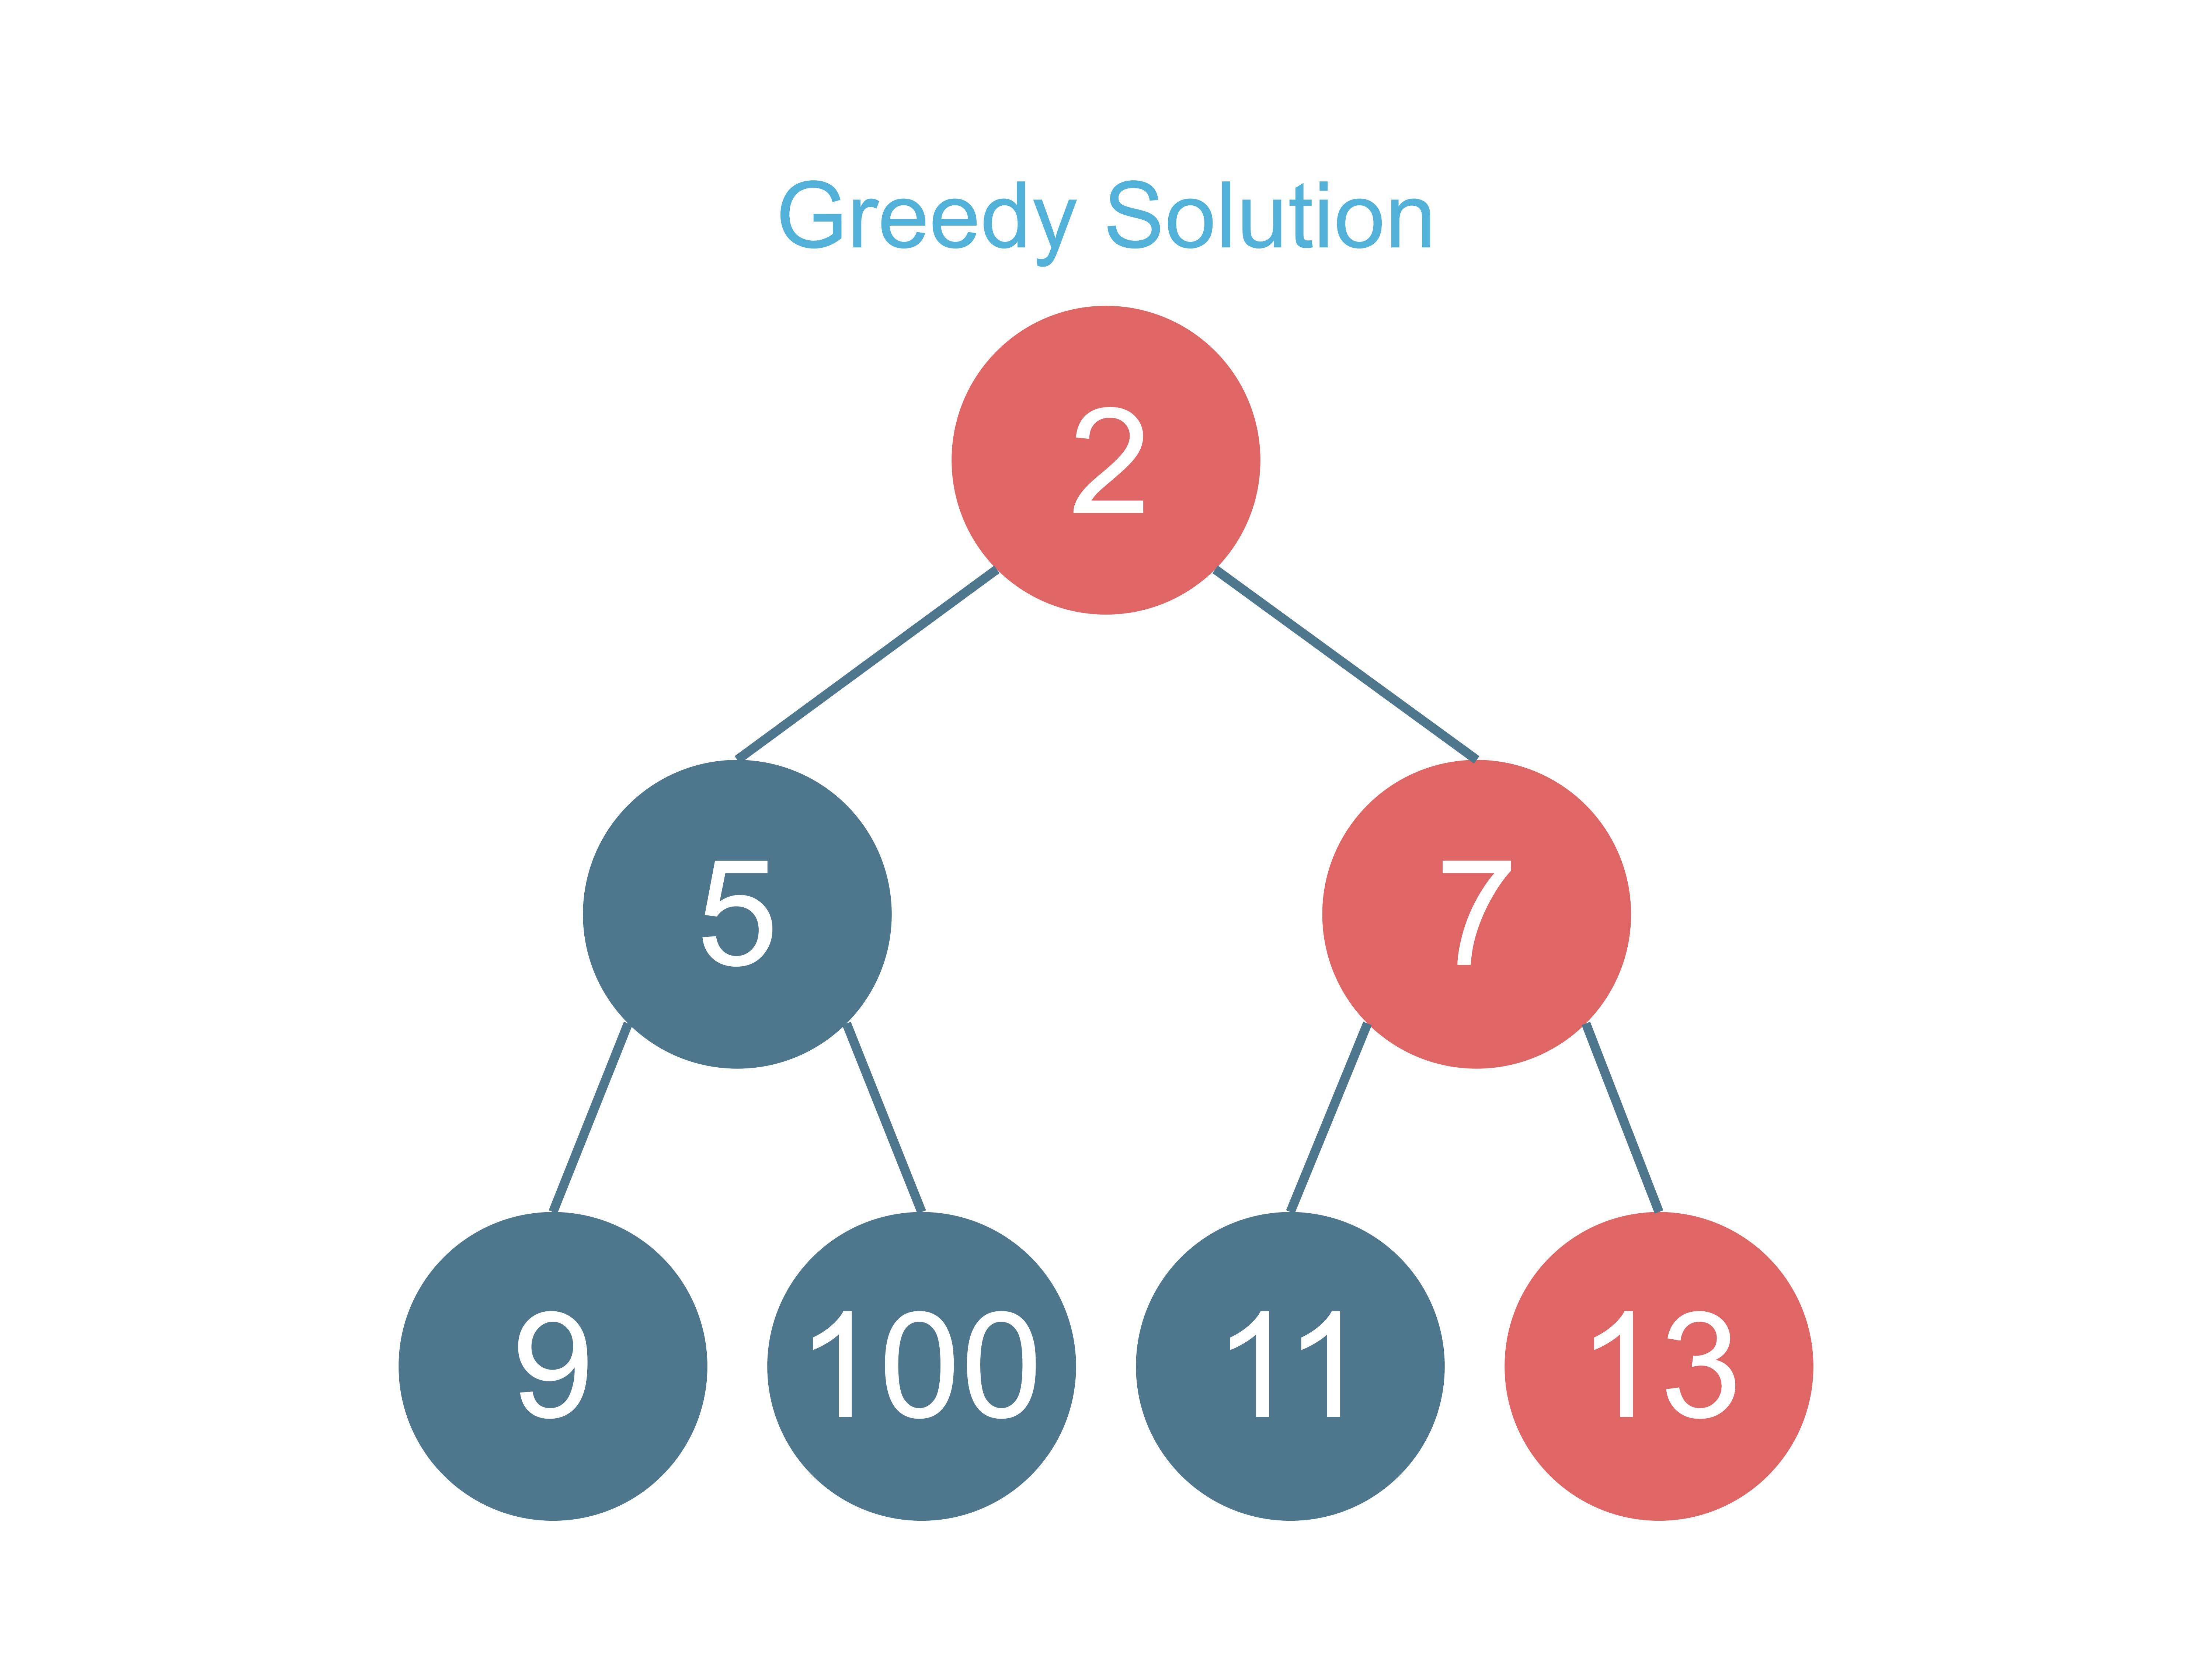
\includegraphics[width=0.5\textwidth,keepaspectratio]{Images/greedy-solution.jpg}
            \caption{An example where the greedy solution results in a suboptimal decision. The greedy choice would be to start at 2, choose 7, then choose 13, for a sum of 22. The optimal solution is instead to start at 2, choose 5, then choose 100, for a sum of 107.}
            \label{fig:greedy-bad}
        \end{figure}

        While greedy algorithms offer simplicity and efficiency, they are susceptible to local optima and may fail to reach the global optimum. The primary limitations of greedy approaches include:

        \begin{itemize}
            \item \textbf{Short-sighted Decision Making:} Greedy algorithms prioritize immediate gains without anticipating future consequences, potentially overlooking better long-term solutions.
        
            \item \textbf{Lack of Backtracking:} Once a decision is made in a greedy algorithm, it cannot be revised or reconsidered in light of subsequent information, leading to suboptimal outcomes in complex problems.
        \end{itemize}
        
        Despite their drawbacks, greedy algorithms serve as foundational techniques in algorithm design and optimization. They provide valuable insights into problem-solving strategies and can serve as building blocks for more sophisticated algorithms and heuristic methods.
        
        \subsection{Dynamic Programming}
        Dynamic programming is a powerful optimization technique used to solve complex problems by breaking them down into simpler subproblems and storing the solutions to these subproblems to avoid redundant computations. It is particularly effective for problems that exhibit optimal substructure and overlapping subproblems, allowing for efficient computation of the optimal solution.
        
        Dynamic programming involves the following key concepts:

        \begin{enumerate}
            \item \textbf{Optimal Substructure:} The optimal solution to a problem can be constructed from optimal solutions to its subproblems. In other words, the problem can be decomposed into smaller subproblems, and the optimal solution can be derived recursively.
        
            \item \textbf{Memoization:} Dynamic programming uses memoization to store the solutions to subproblems in a table (often referred to as a memoization table or DP table). This avoids redundant computations by retrieving precomputed solutions when needed.
        
            \item \textbf{Bottom-Up or Top-Down Approach:} Dynamic programming can be implemented using either a bottom-up approach (iterative) or a top-down approach (recursive with memoization). The choice of approach depends on the problem structure and preferred implementation style.
        \end{enumerate}
        
        One classic example of dynamic programming is the 0/1 Knapsack Problem, where the goal is to maximize the total value of items that can be included in a knapsack without exceeding its weight capacity. The problem exhibits optimal substructure, as the optimal solution to the problem can be constructed from the optimal solutions to subproblems (i.e., deciding whether to include each item in the knapsack).
        
        The dynamic programming approach to solving the 0/1 Knapsack Problem involves constructing a DP table where each entry represents the maximum value that can be obtained with a certain capacity of the knapsack and a subset of the items. By systematically filling out this table based on recursive relationships between subproblems, the optimal solution to the Knapsack Problem can be efficiently computed.

        This example showcases the advantages of a dynamic programming approach for solving the knapsack problem, but in general, dynamic programming offers several advantages:

        \begin{itemize}
            \item \textbf{Efficiency:} By storing precomputed solutions to subproblems, dynamic programming avoids redundant computations and significantly reduces computational complexity.
        
            \item \textbf{Versatility:} Dynamic programming can be applied to a wide range of optimization problems, including sequence alignment, shortest path problems, and resource allocation.
        
            \item \textbf{Optimality:} When applied correctly, dynamic programming guarantees finding the optimal solution to the problem, given the problem's structure and constraints.
        \end{itemize}
        
        Dynamic programming is a fundamental technique in algorithm design and optimization, providing a systematic approach to solving complex problems efficiently. Understanding the principles and applications of dynamic programming is essential for developing effective optimization strategies and algorithms.

        \subsection{Metaheuristic Approaches: Genetic Algorithms, Simulated Annealing}
        Genetic algorithms (GAs) and simulated annealing (SA) are powerful metaheuristic optimization techniques inspired by evolutionary biology and thermodynamics, respectively. GAs emulate natural selection and genetic evolution through selection, crossover, and mutation operators to efficiently explore and exploit solution spaces. SA mimics metallurgical annealing, using temperature parameters to probabilistically navigate the solution space and escape local optima. This section explores the principles and applications of GAs and SA in optimization, examining genetic algorithms' representation of solutions within populations and simulated annealing's temperature-based exploration. Through a comparative analysis, we highlight the strengths, limitations, and diverse applications of these metaheuristic approaches in addressing complex optimization problems across various domains.

        \subsubsection{Genetic Algorithms}
        Genetic algorithms (GAs) are a class of metaheuristic optimization algorithms inspired by the principles of natural selection and genetics. The concept of genetic algorithms was introduced by John Holland in the 1960s and further popularized by Goldberg in the 1980s. Genetic algorithms mimic the process of natural evolution to search for optimal solutions to complex problems.

        Genetic algorithms operate based on several key concepts. Firstly, solutions to optimization problems are represented as individuals (chromosomes) within a population. Each individual encodes a potential solution using a string of symbols, such as binary strings or real-valued vectors. The genetic representation allows for a diverse exploration of the solution space.
        
        Selection is a fundamental aspect of genetic algorithms. Fitness-based selection mechanisms are employed to determine which individuals (solutions) will contribute to the next generation. Individuals with higher objective function values are favored for reproduction, increasing their likelihood of passing on favorable traits to offspring.
        
        Reproduction in genetic algorithms involves genetic operators such as crossover and mutation. Crossover combines genetic material from two parent individuals to produce offspring with traits inherited from both parents. Mutation introduces random changes to individual chromosomes, allowing for exploration of new solution spaces and maintaining diversity within the population.
        
        Genetic algorithms maintain a population of individuals across generations. New generations are created through selection, crossover, and mutation, allowing the algorithm to explore and exploit the solution space over time. The process continues until a termination criterion is met, such as reaching a maximum number of generations or achieving a satisfactory solution quality.
        
        The pseudocode for a simple genetic algorithm is outlined below:
        
        \begin{algorithm}[!h]
            \DontPrintSemicolon
            \caption{GeneticAlgorithm}
            \label{alg:gaOptimize}
            \KwResult{Optimal found solution vector $solution$ and solution fitness $d$}
            Let $generations$ be an arbitrary integer $> 0$\;
            Let $populationSize$ be an arbitrary integer $> 0$\;
            Let $mutationRate$ be an arbitrary real number $0 \leq mutationRate \leq 1$\;
            Build initial population by generating $population$ random solutions\;
            \ForEach{element $\in$ initial population}
            {
                Evaluate each member of the initial population\; 
            }
            $population \gets $ initial population\;
            \ForEach{$i\in generations$}
            {
                $newPopulation \gets \{\}$\;
                \ForEach{$j \in populationSize$}
                {
                    $parent1 \gets $ result of Algorithm \ref{alg:gaTourn}: \texttt{TournamentSelection}\;
                    $parent2 \gets $ result of Algorithm \ref{alg:gaTourn}: \texttt{TournamentSelection}\;
                    $child \gets$ result of Algorithm \ref{alg:gaCross}: \texttt{Crossover}\;
                    Let $r$ be a real number $0\leq r \leq 1$ that is randomly generated\;
                    \If{$r \leq mutationRate$}
                    {
                        $child\gets $ result of Algorithm \ref{alg:mutate}: \texttt{Mutate}\;
                    }
                    Evaluate $child$;
                    Add $child$ to $newPopulation$\;
                }
                $population \gets newPopulation$\;
            }
            \Return{best solution from $population$}
        \end{algorithm}
        
        \begin{algorithm}[!h]
            \DontPrintSemicolon
            \caption{TournamentSelection(population)}
            \label{alg:gaTourn}
            \KwData{All members of the current $population$}
            \KwResult{Best solution out of $tournamentSize$ randomly selected solutions}
            Let $tournamentSize$ be an arbitrary integer $> 0$\;
            \ForEach{$i \in tournamentSize$}
            {
                Get random solution from $population$\;
            }
            \Return{best $solution$ from the random solutions picked}
        \end{algorithm}
        
        \begin{algorithm}[!h]
            \DontPrintSemicolon
            \caption{Crossover(parent1, parent2}
            \label{alg:gaCross}
            \KwData{$parent1$ and $parent2$ are parents to perform crossover upon}
            \KwResult{Best solution after performing single point crossover between $parent1$ and $parent2$}
            $n\gets$ number of elements in $parent1$\;
            Randomly generate crossover point $p$ such that $0\leq p \leq n$\;
            $child1\gets\{\}$\;
            $child2\gets\{\}$\;
            Select first $p$ elements in $parent1$ and add to $child1$\;
            Fill $n - p$ remaining elements of $child1$ from $parent2$ such that no element of $child1$ is repeated\;
            Select first $p$ elements in $parent2$ and add to $child2$\;
            Fill $n - p$ remaining elements of $child2$ from $parent1$ such that no element of $child2$ is repeated\;
            \Return{best solution from the set \{parent1, parent2, child1, child2\}}
            
        \end{algorithm}
        
        \begin{algorithm}[!h]
            \DontPrintSemicolon
            \caption{Mutate(child)}
            \label{alg:mutate}
            \KwData{$child$ to be mutated}
            \KwResult{Mutated $child$}
            $n\gets$ number of elements in $child$\;
            $index1\gets$ random number such that $0\leq index1\leq n$\;
            $index2\gets$ random number such that $0 \leq index2\leq n$ and $index1\neq index2$\;
            Swap elements at $index1$ and $index2$ of child\;
            \Return{child}\;
        \end{algorithm}

        \newpage
        
        Genetic algorithms offer several advantages and find applications in diverse domains. Firstly, GAs excel at global search and can effectively explore large solution spaces to locate global optima in complex optimization problems. Secondly, genetic algorithms are versatile and can be applied to various optimization problems, including function optimization, feature selection, scheduling, and machine learning. Lastly, genetic algorithms are robust against local optima due to their stochastic nature and population-based approach, allowing them to escape suboptimal solutions and converge towards optimal or near-optimal solutions.
        
        In summary, genetic algorithms represent a powerful optimization approach based on evolutionary principles. By leveraging selection, crossover, and mutation, genetic algorithms efficiently explore and exploit solution spaces, making them valuable tools for solving complex optimization problems across various domains.

        
        \subsubsection{Simulated Annealing}
        Simulated Annealing is a probabilistic metaheuristic algorithm inspired by the annealing process in metallurgy, where a material is gradually cooled to reach a low-energy state. Simulated Annealing was introduced by Kirkpatrick et al. in 1983 \cite{kirkpatrick1983optimization} and mimics the stochastic behavior of atoms in a cooling system. By allowing occasional uphill moves, controlled by a temperature parameter, Simulated Annealing can navigate uphill in the solution space to escape local optima and converge towards optimal or near-optimal solutions.

        The Simulated Annealing algorithm relies on a temperature schedule, neighborhood exploration, acceptance criteria, and a cooling schedule. The algorithm must track a temperature parameter that controls the probability of accepting worse solutions. The temperature decreases over time according to a predefined cooling schedule, typically exponential or logarithmic, simulating the annealing process. Higher temperatures facilitate exploration by allowing uphill moves, while lower temperatures encourage exploitation by favoring downhill moves. At each iteration, Simulated Annealing generates neighboring solutions by applying local modifications to the current solution. Common neighborhood structures include 2-opt, 3-opt, or k-opt moves in the context of the TSP. Simulated Annealing probabilistically accepts or rejects candidate solutions based on their quality and the current temperature. Moves that improve the objective function are always accepted, while worse moves are accepted with a probability determined by some criterion, which relates the change in objective function value to the current temperature. Finally, the cooling schedule dictates the rate at which the temperature decreases over iterations. A slower cooling schedule allows for more exploration in the early stages of the search, while a faster cooling schedule intensifies exploitation towards the later stages. The choice of cooling schedule impacts the algorithm's convergence behavior and solution quality.

        Simulated Annealing operates iteratively, simulating the annealing process through a sequence of temperature-dependent transformations. At each iteration, the algorithm explores neighboring solutions and probabilistically accepts or rejects moves based on their impact on the objective function and the current temperature. As the temperature decreases over time, the likelihood of accepting worse solutions diminishes, leading to convergence towards a global optimum.
        
        \begin{algorithm}[!h]
            \DontPrintSemicolon
            \caption{Simulated Annealing}
            \label{alg:anneal}
            \KwData{$initial\_solution$ is the seed solution, $initial\_temperature$ is the starting temperature of the solution, $cooling\_schedule$ is the rate of temperature decrease}
            \KwResult{}
        
            $current\_solution\gets initial\_solution$\;
            $temperature \gets initial\_temperature$\;
            \While{$temperature > 0$}
            {
                $new\_solution \gets$ some neighbor of $current\_solution$\;
                $delta\_cost \gets$ $objective(new\_solution) - objective(current\_solution)$\;
                \If{$delta\_cost < 0$ or $rand < e^{\frac{-delta\_cost}{temperature}}$}
                {
                    $current\_solution\gets new\_solution$\;
                }
                $temperature\gets cooling(temperature)$\;
            }
            \Return{$current\_solution$}
        \end{algorithm}
        
        \begin{figure}[h]
            \centering
            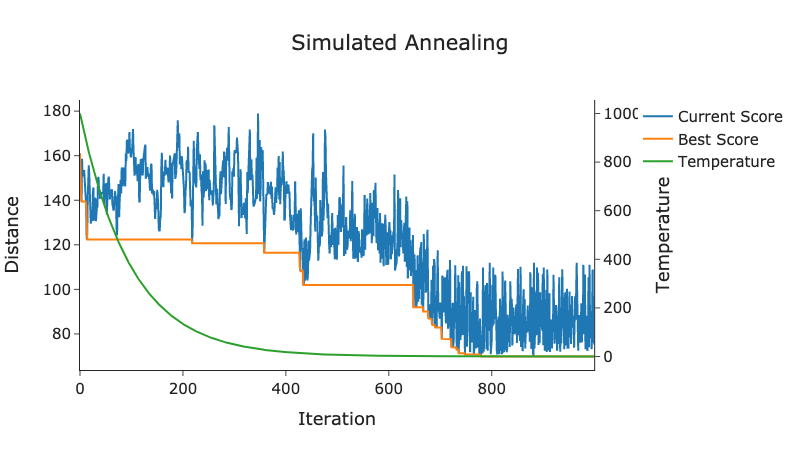
\includegraphics[width=1\textwidth,keepaspectratio]{Images/SA.png}
            \caption{Sample of the Simulated Annealing algorithm improving a solution to the TSP over 1000 iterations}
            \label{fig:bandb}
        \end{figure}
        \newpage
        Simulated Annealing offers a powerful and versatile approach to optimization by emulating the annealing process in metallurgy. In the figure above we can see an example implementation of Simulated Annealing where the temperature of the system decreases exponentially. The current score increases and decreases wildly in the first few hundred iterations, but as the temperature decreases the solution starts to converge on an optimal solution. The best score started at \~160, and after \~700 iterations it had decreased by about 50. Once the temperature fell enough, the algorithm was able to improve the solution by roughly the same delta of 50 while only taking around 75 iterations. This shows how the gradual cooling of the system allows the system to explore many solutions initially and converge as the iterations increase.
        

    \section{Parallel Optimization Techniques}
    In the realm of combinatorial optimization, leveraging parallel computing techniques has become instrumental in addressing complex problems efficiently. This section explores various parallelization strategies and technologies aimed at accelerating the solution process for combinatorial optimization problems.
    
        \subsection{Parallelization Strategies for Combinatorial Problems}

        Combinatorial optimization problems, such as the Traveling Salesman Problem and the Knapsack Problem, often involve exploring vast solution spaces to identify optimal or near-optimal solutions. Parallelization strategies offer effective means to distribute computational tasks across multiple processing units, accelerating solution discovery and improving scalability\cite{755612}. Problems such as these are characterized by their discrete decision variables and complex solution spaces, benefit from parallelization strategies that distribute computational tasks efficiently. This section explores two fundamental approaches to parallelization: task parallelism and data parallelism.

        \subsubsection{Task Parallelism}
            Task parallelism involves decomposing optimization tasks into independent subtasks that can be executed concurrently by multiple processing units. In the context of combinatorial problems, task parallelism is particularly effective for algorithms with inherently parallelizable components, such as search algorithms and divide-and-conquer approaches.

            One common application of task parallelism is in parallel branch-and-bound algorithms for solving optimization problems with discrete decision variables, such as integer programming. In these algorithms, different branches of the search tree representing potential solutions can be explored simultaneously by separate processors or threads. Each processor works on a distinct subproblem, searching for promising solutions and pruning unpromising branches based on global bounds or constraints.
        
            Task parallelism requires careful workload distribution and synchronization mechanisms to ensure efficient use of computational resources and avoid redundant computations. Load balancing techniques, dynamic task scheduling, and efficient communication protocols are essential for maximizing parallel algorithm performance and scalability.

        \subsubsection{Data Parallelism}
            Data parallelism involves distributing data across multiple processing units, with each unit performing the same computation on different subsets of data simultaneously. This approach is well-suited for algorithms that can process large datasets in parallel, such as matrix operations and evolutionary algorithms.

            In the context of combinatorial optimization, data parallelism can be applied to parallel genetic algorithms where multiple populations of candidate solutions evolve concurrently. Each population undergoes genetic operations like crossover and mutation independently, and the best solutions from different populations are periodically exchanged to facilitate diversity and exploration.
        
            Data parallelism requires efficient data partitioning strategies to distribute data evenly across processing units and minimize communication overhead. Techniques like SIMD (Single Instruction, Multiple Data) programming and parallel reduction operations can be employed to leverage the parallel processing capabilities of modern hardware architectures.

        \begin{figure}[h]
            \centering
            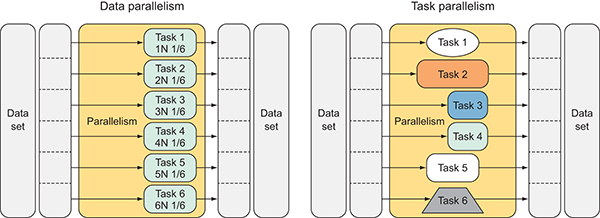
\includegraphics[width=1\textwidth,keepaspectratio]{Images/parallelisim.png}
            \caption{Data parallelism involves executing the same function simultaneously across multiple elements within a data set. In contrast, task parallelism entails executing multiple and potentially different functions concurrently across either the same or different data sets.}
            \label{fig:data-task-parallelism}
        \end{figure}

        \subsubsection{Summary}
            Task parallelism and data parallelism are powerful strategies for accelerating the solution process of combinatorial optimization problems. Task parallelism decomposes complex tasks into independent subtasks, enabling concurrent execution and efficient workload distribution. Data parallelism leverages parallel processing units to operate on different subsets of data simultaneously, enhancing scalability and performance for algorithms that exhibit inherent data parallelism.

        By understanding and implementing task and data parallelism effectively, researchers and practitioners can leverage parallel computing resources to tackle large-scale combinatorial optimization problems efficiently. The choice of parallelization strategy depends on the nature of the problem, available computational resources, and desired optimization objectives, highlighting the importance of tailored parallelization techniques for diverse application domains.

        \subsection{Leveraging GPUs for Parallel Processing}
        GPUs have emerged as powerful platforms for accelerating parallel computations due to their highly parallel architecture and specialized processing capabilities. Integrating GPUs into combinatorial optimization algorithms enables significant speedups and efficiency gains compared to traditional CPU-based approaches. This section explores the utilization of GPUs, focusing on the CUDA programming model and effective parallel algorithm design for combinatorial optimization.

        \subsubsection{CUDA Programming Model}
            NVIDIA's CUDA programming model provides a powerful framework for harnessing the parallel processing capabilities of GPUs. CUDA enables developers to write parallel algorithms that execute efficiently on GPU cores, leveraging massive parallelism for computationally intensive tasks.
            
            Key features of the CUDA programming model include:

            \begin{itemize}
                \item \textbf{Thread Hierarchy:} CUDA organizes computations into a hierarchy of threads, blocks, and grids. Threads execute in parallel within a block, and multiple blocks can be executed concurrently within a grid.
            
                \item \textbf{Shared Memory:} CUDA allows threads within the same block to share data through fast on-chip shared memory, reducing memory access latency and enhancing communication between threads.
            
                \item \textbf{Kernel Functions:} Kernel functions are executed on the GPU and can be launched with specific thread block and grid configurations. This flexibility enables fine-grained control over parallel execution.
            \end{itemize}
            
            Developers utilize CUDA to parallelize algorithms by identifying parallelizable tasks, mapping them to CUDA kernel functions, and optimizing memory access patterns for efficient GPU utilization. CUDA programming requires understanding GPU architecture, memory hierarchy, and thread coordination to maximize performance and scalability.
            
        \subsubsection{Parallel Algorithm Design for GPUs}

            Designing parallel algorithms for GPUs involves restructuring optimization algorithms to exploit GPU parallelism effectively. Effective parallel algorithm design considers workload distribution, memory access patterns, and communication overhead to achieve optimal performance.
    
            Strategies for parallel algorithm design on GPUs include:

            \begin{itemize}
                \item \textbf{Data Decomposition:} Partitioning data to maximize data parallelism and minimize data dependencies. Techniques like tiling and loop unrolling optimize memory access patterns and reduce memory contention.
            
                \item \textbf{Thread Synchronization:} Managing thread synchronization and communication to avoid race conditions and ensure consistent computation results. CUDA provides synchronization primitives like barriers and atomic operations for inter-thread communication.
            
                \item \textbf{Memory Optimization:} Minimizing global memory accesses and leveraging shared memory for data reuse and inter-thread communication. Optimizing memory access patterns and reducing memory overhead are critical for maximizing GPU performance.
            \end{itemize}
            
            By optimizing algorithm design for GPU architectures, developers can achieve significant speedups and scalability for combinatorial optimization problems. Parallel algorithm design involves balancing computational complexity, memory efficiency, and parallelization overhead to fully exploit the computational power of GPUs.

        \subsubsection{Summary}
        Leveraging GPUs for parallel processing in combinatorial optimization requires proficiency in the CUDA programming model and effective parallel algorithm design. CUDA provides a versatile platform for implementing parallel algorithms, while parallel algorithm design focuses on optimizing data decomposition, thread synchronization, and memory usage for efficient GPU utilization.

        Understanding the nuances of GPU programming and parallel algorithm design is essential for developing high-performance solutions to complex optimization problems. By harnessing the computational capabilities of GPUs, researchers and practitioners can accelerate solution discovery and achieve scalability for large-scale combinatorial optimization tasks.

    \section{CUDA Implementation of Optimization Algorithms}
        The implementation of optimization algorithms using CUDA presents a compelling opportunity to leverage the massive parallel processing capabilities of GPUs for solving computationally intensive problems. Certain optimization problems lend themselves naturally to parallelization, making them ideal candidates for GPU-accelerated algorithms.
        \subsubsection{Parallelizable Optimization Problems}
        Many optimization problems exhibit inherent parallelism due to the independent nature of subtasks or solution components. Combinatorial optimization problems, such as the Traveling Salesman Problem, Knapsack Problem, and Maximum Clique Problem, often involve exploring large solution spaces where parallelization can expedite solution discovery.

        Furthermore, optimization problems that involve iterative search or stochastic methods, such as Ant Colony Optimization and Particle Swarm Optimization, are well-suited for parallelization on GPUs. These algorithms simulate collective behaviors or search processes that can be efficiently parallelized using CUDA's parallel programming model.
        \subsubsection{GPU-Parallelizable Optimization Algorithms}
        Certain optimization algorithms can benefit significantly from GPU parallelization, enabling faster convergence and scalability for large-scale problem instances. Examples of optimization algorithms suitable for GPU parallelization include:

        \begin{itemize}
            \item \textbf{Ant Colony Optimization (ACO):} A metaheuristic inspired by the foraging behavior of ants, ACO involves iterative construction of candidate solutions and pheromone-based communication. The parallelization of ACO on GPUs allows for concurrent exploration of solution spaces and efficient pheromone update operations.
        
            \item \textbf{Particle Swarm Optimization (PSO):} A population-based stochastic optimization technique that simulates the social behavior of particles moving through a search space. GPU-accelerated PSO enables simultaneous evaluation of particle positions and velocities, enhancing exploration and exploitation capabilities.
        
            \item \textbf{Genetic Algorithms (GAs):} Evolutionary algorithms like GAs involve the parallel evaluation and evolution of candidate solutions through genetic operators (e.g., crossover, mutation). GPU parallelization of GAs facilitates rapid evaluation of fitness functions and parallel execution of genetic operations.
        \end{itemize}
        
        \subsubsection{Leveraging CUDA for Optimization}
        Utilizing CUDA for implementing optimization algorithms involves designing efficient parallel algorithms tailored to GPU architectures and leveraging CUDA libraries for optimized computations. CUDA's programming model enables developers to harness thousands of GPU cores for parallel execution, accelerating optimization tasks and enabling scalability to handle large-scale problem instances.
        
        In summary, CUDA implementation of optimization algorithms offers a powerful approach to solving complex optimization problems efficiently. By identifying parallelizable optimization problems, leveraging GPU-accelerated algorithms, and utilizing CUDA's programming model and libraries, researchers and practitioners can unlock new capabilities for tackling computationally demanding optimization challenges.
        
        \subsection{Designing Parallel Algorithms for GPUs}
        Designing efficient parallel algorithms for GPUs involves careful consideration of data decomposition, thread coordination, memory optimization, and kernel design. This subsection explores key strategies and techniques for maximizing GPU utilization in optimization algorithms.

        \subsubsection{Data Decomposition}
        Data decomposition is a critical aspect of parallel algorithm design that involves partitioning problem data to maximize data parallelism and minimize data dependencies. Effective data decomposition strategies enable concurrent execution of independent tasks across GPU threads.

        Some of the most common strategies for data decomposition include the following:

        \begin{itemize}
            \item \textbf{Task Distribution:} Dividing the optimization task into smaller subtasks that can be executed independently by GPU threads. For example, in parallel genetic algorithms, different threads can evaluate fitness functions for distinct candidate solutions simultaneously.
        
            \item \textbf{Data Partitioning:} Splitting input data into manageable chunks distributed across GPU threads. Techniques like block-level and grid-level partitioning ensure balanced workload distribution and efficient memory access patterns.
        
            \item \textbf{Load Balancing:} Ensuring uniform distribution of computational workload among GPU threads to maximize GPU utilization and minimize idle time. Dynamic load balancing techniques adjust workload distribution based on thread performance metrics.
        \end{itemize}
        
        Data decomposition is essential for leveraging GPU parallelism effectively, enabling scalable and efficient execution of parallel optimization algorithms on GPUs.
        
        \subsubsection{Thread Coordination}
        Thread coordination involves managing synchronization, communication, and workload distribution among GPU threads to avoid race conditions and ensure coherent computation results. Efficient thread coordination is crucial for optimizing parallel algorithm performance on GPUs.

        To effectively coordinate threads, a few simple strategies are implemented:
        \begin{itemize}
            \item \textbf{Barrier Synchronization:} Using synchronization barriers to coordinate thread execution and enforce ordered operations. Barriers ensure that all threads reach a synchronization point before proceeding to the next phase of computation.

            \item \textbf{Thread Mapping:} Mapping computational tasks to GPU threads to minimize thread divergence and maximize thread utilization. Strategies like thread grouping and warp-level parallelism optimize thread coordination for specific GPU architectures.
        
            \item \textbf{Workload Distribution:} Balancing computational workload across GPU blocks and grids to maximize resource utilization and minimize idle thread cycles. Dynamic workload distribution techniques adapt to changing computational requirements during algorithm execution.
        \end{itemize}
        
        \subsubsection{Memory Optimization}
        Memory optimization focuses on leveraging GPU memory hierarchy, including global memory, shared memory, and registers, to optimize memory access patterns and minimize memory latency. Effective memory management is essential for maximizing GPU performance in parallel algorithms.

        To optimize the memory usage and memory patterns to maximize GPU performance, the main strategies include:

        \begin{itemize}
            \item \textbf{Shared Memory Usage:} Exploiting fast on-chip shared memory for inter-thread communication and data sharing within GPU blocks. Efficient use of shared memory reduces memory access latency and minimizes global memory overhead.
        
            \item \textbf{Memory Coalescing:} Aligning memory access patterns to maximize memory coalescing and minimize memory contention. Techniques like memory padding and data alignment optimize memory transactions for efficient GPU utilization.
        
            \item \textbf{Texture and Constant Memory:} Leveraging texture and constant memory caches for read-only data access and caching frequently accessed data. Optimizing memory access patterns enhances memory bandwidth utilization and reduces memory latency.
        \end{itemize}
        
        Effective memory optimization enhances memory bandwidth utilization and reduces memory access latency, improving overall performance of parallel algorithms on GPUs.
        
        \subsubsection{Kernel Design}
        Kernel design involves structuring CUDA kernel functions to efficiently execute parallel tasks on GPU cores. Optimizing kernel design maximizes parallelism and minimizes execution overhead, enhancing algorithm performance on GPUs.

        Some strategies for optimizing the design of the kernels include:

        \begin{itemize}
            \item \textbf{Loop Unrolling:} Unrolling loops within kernel functions to expose more parallelism and reduce loop overhead. Loop unrolling minimizes control divergence and enhances instruction-level parallelism.
        
            \item \textbf{Memory Coalescing Optimization:} Aligning memory access patterns to maximize memory coalescing and minimize memory transactions. Optimizing memory access within kernel functions improves memory throughput and reduces memory latency.
        
            \item \textbf{Warp-Level Parallelism:} Leveraging warp-level execution to maximize GPU core utilization and minimize thread divergence. Strategies like conditional execution and predication enhance warp efficiency and parallel execution.
        \end{itemize}
        
        By optimizing kernel design, developers can achieve maximum utilization of GPU resources and enhance the performance of parallel optimization algorithms.
        
        \subsubsection{Summary}
        Designing parallel algorithms for GPUs involves a holistic approach to data decomposition, thread coordination, memory optimization, and kernel design. By leveraging these strategies effectively, developers can harness the massive parallelism of GPUs to accelerate optimization tasks and achieve scalability for large-scale problem instances.

        Integrating data decomposition, thread coordination, memory optimization, and kernel design techniques enables efficient utilization of GPU resources and enhances the performance of parallel optimization algorithms. Understanding these key aspects of parallel algorithm design is essential for developing high-performance GPU-accelerated solutions to complex optimization challenges.

        \subsection{Utilizing CUDA Libraries for Optimization}
        CUDA libraries provide specialized functionalities and optimized routines for accelerating various optimization tasks on GPUs. This section explores key CUDA libraries, including cuBLAS, cuSPARSE, cuDNN, and Thrust, and their applications in optimizing optimization algorithms.

        
        \subsubsection{cuBLAS (CUDA Basic Linear Algebra Subroutines)}
        
        cuBLAS is a CUDA-accelerated library that provides optimized routines for basic linear algebra operations, including matrix-vector multiplication, matrix-matrix multiplication, and matrix factorization. It leverages GPU parallelism to accelerate linear algebra computations essential for many optimization algorithms.
        
        \textbf{Key Features and Applications of cuBLAS:}

        \begin{itemize}
            \item Accelerated matrix operations for optimization algorithms such as gradient descent, linear programming, and eigenvalue computations.
        
            \item High-performance implementations of BLAS (Basic Linear Algebra Subprograms) routines optimized for GPU architectures.
        
            \item Support for batched operations and custom data layouts to accommodate diverse optimization tasks.
        \end{itemize}
        
        cuBLAS enables developers to leverage GPU-accelerated linear algebra primitives to accelerate optimization algorithms and improve computational efficiency.

        \subsubsection{cuSPARSE}
        cuSPARSE is a CUDA-accelerated library for sparse matrix computations, offering optimized routines for sparse matrix-vector multiplication, sparse matrix-matrix multiplication, and sparse matrix factorization. It facilitates efficient handling of large-scale sparse matrices commonly encountered in optimization problems.
        
        \textbf{Key Features and Applications of cuSPARSE:}
        \begin{itemize}
            \item Accelerated sparse matrix operations for optimization algorithms requiring sparse data representations.
        
            \item Support for compressed sparse row (CSR) and compressed sparse column (CSC) formats to efficiently store and manipulate sparse matrices.
        
            \item High-performance implementations of sparse linear algebra routines optimized for GPU architectures.
        \end{itemize}
        
        cuSPARSE provides essential tools for optimizing optimization algorithms that involve sparse data structures, enhancing scalability and performance on GPU platforms.
        
        \subsubsection{cuDNN (CUDA Deep Neural Network)}
        cuDNN is a CUDA-accelerated library specifically designed for deep learning tasks, offering optimized routines for neural network training and inference. While primarily used in deep learning applications, cuDNN can be leveraged for optimizing optimization algorithms based on neural network techniques.
        
        \textbf{Key Features and Applications of cuDNN:}
        \begin{itemize}
            \item Accelerated implementations of convolutional neural network (CNN) operations, recurrent neural network (RNN) operations, and other deep learning primitives.
        
            \item Support for optimized memory management, tensor operations, and activation functions.
        
            \item Integration with popular deep learning frameworks like TensorFlow and PyTorch for seamless GPU acceleration of optimization algorithms.
        \end{itemize}
        
        cuDNN provides GPU-accelerated tools for implementing advanced optimization algorithms based on neural network architectures, enabling rapid experimentation and deployment of GPU-accelerated solutions.
        
        \subsubsection{Thrust}
        Thrust is a parallel algorithms library for CUDA that provides high-level abstractions and optimized primitives for GPU-accelerated computations. It simplifies the development of parallel optimization algorithms by offering a familiar STL-like interface and efficient parallel implementations.
        
        \textbf{Key Features and Applications of Thrust:}
        \begin{itemize}
            \item Abstractions for parallel algorithms such as sorting, reduction, scan, and transform.
        
            \item Seamless integration with CUDA kernels and GPU memory management.
        
            \item Optimized implementations of common parallel patterns for accelerating optimization tasks.
        \end{itemize}
        
        Thrust streamlines the development of GPU-accelerated optimization algorithms by providing high-level abstractions and optimized primitives, enabling rapid prototyping and deployment.

        \subsubsection{Summary}
        Leveraging CUDA libraries such as cuBLAS, cuSPARSE, cuDNN, and Thrust empowers developers to accelerate optimization algorithms on GPUs efficiently. These libraries offer specialized functionalities and optimized routines tailored for GPU architectures, enhancing performance, scalability, and productivity in developing GPU-accelerated solutions to complex optimization challenges.
        
        Integrating CUDA libraries into optimization algorithm implementations enables researchers and practitioners to exploit the computational capabilities of GPUs effectively, achieving significant speedups and scalability for large-scale optimization problems. Understanding the features and applications of CUDA libraries is essential for harnessing GPU-accelerated computing in optimizing optimization algorithms across diverse domains.

    \section{Challenges and Future Directions in Parallel Optimization}
    Parallel optimization techniques leveraging GPUs offer significant performance benefits but also pose challenges that need to be addressed for broader adoption and improved efficiency. This section explores key challenges and emerging trends in parallel optimization, along with future directions for advancing GPU-accelerated optimization algorithms.
    
        \subsection{Scalability Issues and Load Balancing}
        Scalability is a critical consideration in parallel optimization, especially when dealing with large-scale problem instances. This subsection explores key scalability challenges and strategies for load balancing to optimize resource utilization and minimize computational overhead.
        
        \subsubsection{Scalability Challenges}
            Scalability challenges in parallel optimization arise from the increasing complexity and size of problem instances, leading to limitations in memory capacity, communication overhead, and computational bottlenecks. Common scalability challenges include:
            \begin{itemize}
                \item \textbf{Memory Constraints:} Large problem instances may exceed the available GPU memory, necessitating efficient memory management strategies such as data partitioning and memory pooling. For example, when considering all 1.9 million cities in the world as an instance of the TSP, an adjacency matrix that represents the distances between each city would require $\left(1.9e06\right)^2\text{ entries} \times 4 \text{ bytes per entry} = 14,440,000,000,000 \text{ bytes} = 14.44 \text{ TeraBytes}$ just to represent the problem. 
            
                \item \textbf{Communication Overhead:} Coordinating data transfer and synchronization between GPU threads and processing units can introduce communication overhead, impacting overall performance and scalability.
            
                \item \textbf{Computational Bottlenecks:} Certain optimization algorithms may exhibit inherent computational bottlenecks that limit scalability, such as dependency chains or sequential processing steps.
            \end{itemize}
            
            Addressing scalability challenges requires innovative approaches to optimize resource utilization, mitigate communication overhead, and enhance parallelism across GPU cores.
        \subsubsection{Load Balancing Strategies}
        Effective load balancing is essential for maximizing parallelism and optimizing resource utilization in GPU-accelerated optimization algorithms. This subsection explores strategies for load balancing to distribute computational workload evenly across GPU threads and processing units:
        \begin{itemize}
            \item \textbf{Dynamic Workload Distribution:} Implementing dynamic load balancing techniques to adaptively distribute computational tasks based on workload characteristics and resource availability.
        
            \item \textbf{Task Partitioning:} Partitioning computational tasks into smaller subtasks that can be executed independently by GPU threads, optimizing parallelism and minimizing idle time.
        
            \item \textbf{Workload Monitoring and Adjustment:} Continuously monitoring workload distribution and performance metrics to dynamically adjust task assignments and optimize resource utilization.
        \end{itemize}
        By implementing efficient load balancing strategies, developers can achieve optimal parallelism and scalability in GPU-accelerated optimization algorithms, improving overall performance and accelerating solution discovery for complex problem instances.
        \subsubsection{Summary}
        Addressing scalability challenges and implementing effective load balancing strategies are key factors in advancing parallel optimization on GPUs. Overcoming scalability limitations and optimizing resource utilization will drive innovation and enable efficient solution discovery for large-scale optimization problems.

        Understanding the intricacies of scalability and load balancing is essential for developing high-performance GPU-accelerated optimization algorithms and harnessing the full potential of parallel computing in optimizing complex optimization tasks across diverse application domains.

        \subsection{Hybrid CPU-GPU Approaches}
        Hybrid CPU-GPU approaches leverage the complementary strengths of CPUs and GPUs to optimize optimization algorithms efficiently. This subsection explores key considerations and strategies for integrating CPUs and GPUs in parallel optimization.
        \subsubsection{Complementary Computing}
        One of the key advantages of hybrid CPU-GPU computing is the complementary nature of CPU and GPU architectures:
        \begin{itemize}
            \item \textbf{CPU Strengths:} CPUs excel at handling sequential tasks, complex control flow, and tasks requiring high single-thread performance.
        
            \item \textbf{GPU Strengths:} GPUs are highly efficient for parallelizable computations, capable of processing large amounts of data simultaneously using thousands of cores.
        \end{itemize}
        By leveraging both CPU and GPU architectures, developers can exploit complementary computing capabilities to accelerate optimization algorithms and achieve optimal performance.
        
        \subsubsection{Data Transfer and Synchronization}
        Integrating CPUs and GPUs in hybrid computing presents challenges related to data transfer and synchronization:
        \begin{itemize}
            \item \textbf{Data Transfer Overhead:} Transferring data between CPUs and GPUs incurs overhead due to memory transfer latency and synchronization costs. Minimizing data movement and optimizing data transfer protocols are essential for reducing overhead.
        
            \item \textbf{Task Synchronization:} Coordinating tasks between CPUs and GPUs requires efficient synchronization mechanisms to ensure coherence and consistency in computational results.
        \end{itemize}
        Addressing data transfer and synchronization challenges is crucial for optimizing hybrid CPU-GPU computing and maximizing overall efficiency.
        \subsubsection{Task Partitioning}
        Effective task partitioning is essential for leveraging hybrid CPU-GPU architectures efficiently:
        \begin{itemize}
            \item \textbf{Task Offloading:} Identifying parallelizable tasks suitable for GPU acceleration and offloading them to GPUs, while assigning sequential or control-intensive tasks to CPUs.
        
            \item \textbf{Dynamic Workload Distribution:} Dynamically partitioning computational tasks based on workload characteristics and resource availability to maximize resource utilization and minimize idle time.
        \end{itemize}
        Optimizing task partitioning enables developers to harness the combined processing power of CPUs and GPUs effectively, accelerating solution discovery for complex optimization problems.
        \subsubsection{Summary}
        Hybrid CPU-GPU approaches offer a promising avenue for optimizing optimization algorithms by combining the strengths of both CPU and GPU architectures. Addressing challenges and implementing strategies for efficient integration of CPUs and GPUs will drive innovation and enable efficient solution discovery for large-scale optimization problems.

        Understanding the benefits, challenges, and strategies of hybrid CPU-GPU computing is essential for researchers and practitioners seeking to leverage heterogeneous computing architectures for accelerating optimization tasks across diverse application domains.

        \subsection{Integrating Deep Learning for Optimization}
        Integrating deep learning techniques into optimization algorithms offers new opportunities for improving solution quality, efficiency, and scalability. This section explores key strategies and applications of deep learning in parallel optimization.
        \subsubsection{Neural Network Architectures}
        Deep learning enables the integration of neural network architectures into optimization algorithms, providing flexible modeling capabilities for complex tasks:
        \begin{itemize}
            \item \textbf{Convolutional Neural Networks (CNNs):} Leveraging CNNs for feature extraction and pattern recognition in optimization tasks requiring image or spatial data analysis.
        
            \item \textbf{Recurrent Neural Networks (RNNs):} Employing RNNs for sequence modeling and time-series analysis in optimization algorithms with temporal dependencies.
        
            \item \textbf{Graph Neural Networks (GNNs):} Utilizing GNNs for modeling graph-structured data in optimization problems involving relational or network-based constraints.
        \end{itemize}
        
        By integrating diverse neural network architectures, developers can design adaptive optimization algorithms capable of handling complex problem structures and diverse data modalities effectively.
        
        \subsubsection{End-to-End Optimization}
        End-to-end optimization pipelines leverage deep learning frameworks to automate solution discovery and optimization processes:
        \begin{itemize}
            \item \textbf{Automated Feature Engineering:} Using deep learning models to automatically extract relevant features from raw data, reducing manual feature engineering efforts and improving model generalization.
        
            \item \textbf{Hyperparameter Optimization:} Employing deep learning-based techniques like Bayesian optimization or reinforcement learning to automate hyperparameter tuning and optimization algorithm selection.
        
            \item \textbf{Reinforcement Learning for Optimization:} Applying reinforcement learning frameworks to learn optimal policies for sequential decision-making in optimization tasks.
        \end{itemize}
        End-to-end optimization pipelines streamline solution discovery and accelerate convergence, enabling rapid experimentation and deployment of optimized solutions.
        \subsubsection{Transfer Learning and Meta-Learning}
        Transfer learning and meta-learning techniques adapt deep learning models to diverse optimization domains and problem instances:

        \begin{itemize}
            \item \textbf{Transfer Learning:} Fine-tuning pre-trained deep learning models on related tasks to accelerate learning and adaptation in new optimization domains.
        
            \item \textbf{Meta-Learning:} Training meta-learners to adapt optimization algorithms to specific problem instances or environments, enabling rapid adaptation and generalization across diverse scenarios.
        
            \item \textbf{Model Compression and Pruning:} Applying model compression techniques to reduce the computational complexity and memory footprint of deep learning models, optimizing performance in resource-constrained environments.
        \end{itemize}
        Integrating transfer learning and meta-learning strategies enhances the adaptability, scalability, and generalization capabilities of deep learning-based optimization algorithms.
        \subsubsection{Summary}
        Integrating deep learning techniques into optimization algorithms opens up exciting possibilities for improving solution discovery and efficiency. Leveraging diverse neural network architectures, implementing end-to-end optimization pipelines, and applying transfer learning/meta-learning strategies enable developers to design adaptive and scalable optimization algorithms capable of addressing complex problem instances across diverse application domains.

        Understanding the applications and implications of deep learning in optimization is essential for researchers and practitioners seeking to harness the power of AI-driven approaches in accelerating solution discovery and optimization tasks.

\pagebreak

\chapter{Methodology and Implementation}

    \section{Setting Up CUDA Development Environment}
    Before any developer begins running CUDA it is essential that they are utilizing an NVIDIA GPU that has a compute capability with the features required for their application. While CUDA has not changed much from one generation of compute capability to the other, there are may important features that have been a part of more recent releases.

    Atomic functions are a good example of a functionality that has frequently changed across compute capability. With a device capable of compute capability 2.0 and higher, 32-bit floating point atomic additions became supported, soon followed by compute capability 6.0 and higher, which introduced 64-bit floating point atomic additions\cite{CPP_GUIDE}.

    Before the installation of the CUDA Toolkit and SDK, it is essential that the host system has installed the graphics drivers from NVIDIA that are compatible with their GPU. Doing so will allow the host system to interact with and successfully install the toolkit. After installing compatible drivers, the CUDA toolkit may be installed. 


    \section{Designing Parallel Optimization Algorithms}
    Given the immense capability of parallel algorithms, it should be of no surprise that so many have been developed since the beginning of distributed computing around the early 1970s. But even these algorithms must follow some basic rules in order for their successful and rapid execution on a GPU. But one must first consider the problem to be solved, existing solutions, and perhaps how to combine conventional aproaches with additional parallel thinking.
    
        \subsection{Algorithm Selection}
        The basic rules involving the parallelizability of an algorithm surround governing the interaction between a GPU core and a location in memory. As a simple rule, every processes on every core should run independently from the other. How this is achieved can be broken down as follows:

        \begin{enumerate}
            \item No two processes should be allowed to alter the same location in memory at the exact same time.
            \item The number of instructions a thread must execute should be fixed for a given input.
            \item Input data should not be calculated while a process is running.
            \item Output data must not be overwritten by another thread.
        \end{enumerate}

        While it is permissible for input data and output data to be in a similar location (for say updating an array by multiplying each index by 2 where each thread gets a single index) this should be generally avoided as the scheduling overhead for such a simple operation may consume more time than required. There are also situations that may arise where input data and output data are the same, and each thread is given a random (possibly repeating) location in memory to manipulate. In which case it becomes possible to violate both rules three and four, however, such an operation may yet experience speedups of parallel execution so long as read and write overlaps are handled with atomic locking, and the likelihood of two threads attempting such overlaps remain low. Regardless of the algorithm, rule one is absolute, and must never be violated.

        Expanding on rule two, problems should not dynamically change. A common programming practice is the use of recursion and runtime stack for traversing data structures until some base case is reached. This should be avoided whenever possible when designing parallel algorithms. The dynamically growing nature of recursive algorithms and the usage of runtime stack can quickly result in overflow as problem sizes are scaled upwards. This also makes synchronization unpredictable and there may be instances where few threads are still searching for the base case while all others have finished and remain idle, resulting in a substantial loss of runtime.


        \subsection{Algorithm Adaptation for GPUs}
        There are many sequential algorithms that can be easily converted to CUDA so long as doing so would not violate the rules in the previous subsection. CUDA's nature of executing on GPUs make them best suited for solving problems involving two and three-dimensional structures; with plenty of support for two and three dimensional pointers. Data may also be flattened into a long, static, one dimensional array for increased execution speed.

        Ideally, problems with a runtime of $O(n^2)$ or larger are best suited for execution on the GPU since each thread may perform $O(n)$ operations. Linear problems may also be considered for improvement on the GPU to attempt to run in logarithmic or constant time, however this is inadvisable for smaller problems. GPUs sacrifice clock speed for cores, making most modern CPUs far more efficient for solving many linear problems. Regardless, in the event of a large linear problem, improvements on the GPU may be considered. 
        
        \subsection{Parallel Data Structures and Memory Management}
        Most algorithms consume a large amount of memory beyond the input and output data. Algorithms have various aspects that must be "remembered" from one step to the other, all of which must be stored in memory. The best way to avoid using more memory than required is to only store on the GPU memory that is required. It is also essential (especially for exceedingly large problems) for data to be periodically renewed. Say there is a 32GB dataset to be processed, but a GPU only has room for 8GB of global memory, it becomes essential to load as much input data as possible, and once that has run out, renew the data from the data set. While not as fast as being able to load it all at once, the limiting factor becomes the device's ability to run though the data.


    \section{Integration of CUDA with Combinatorial Problems}
    Due to the massive solution space of combinatorial problems, GPU architecture's parallel nature makes them best suited to explore a solution space and test the fitness of multiple solutions at a time. Compared to classical approaches which either explore only one to a handful of these possible solutions at a time; massively parallel algorithms make use of the full capability GPUs offer.
    
        \subsection{Mapping Problem Domains to GPU Architecture}
        As mentioned in section 1.4, flooding the GPU is one way to ensure maximum utilization of a GPU. The massive scale of combinatorial problems makes flooding the GPU an intuitive task, as algorithms for solving these seek to explore as many solutions as possible in the shortest amount of time. Certain metaheuristic algorithms for solving combinatorial problems also offer ways to flood a GPU for providing maximum performance of GPU architecture. The next chapter features a project which utilized CUDA with such a metaheurisitic algorithm for flooding the GPU, despite it's approach not necessarily exploring the fitness of every possible solution.
        
        \subsection{Leveraging CUDA Features for Optimization}
        CUDA offers unique features for optimization, including a set of libraries which offer important functionality for execution in parallel. One such library is the cuRAND library which offers a large number of different pseudo random algorithms designed to create distinct random numbers in parallel for the inclusion of stochasticity in data and selection processes\cite{CURAND}. Another parallel library offered in the CUDA toolkit is cuFFT, which provides the Fast Fourier Transform (FFT) accelerated on the GPU for improved runtime beyond a traditional approach\cite{CUFFT}. 


\chapter{Project Evaluation: CUDA-Based Ant Colony Optimization for the TSP}

    \section{Project Overview}
       In the realm of combinatorial optimization, researchers continually seek innovative strategies to address complex problems efficiently. This project focuses on the intersection of combinatorial optimization, parallel computing, and particle swarm intelligence. Specifically, this chapter delves into the intricacies of solving the Traveling Salesman Problem using the Ant Colony Optimization algorithm implemented in parallel with CUDA\footnote{This project was an undertaking performed by the authors of this report. \href{https://github.com/AStruthers2000/TravelingSalesmanProblem_CUDA}{The full code, documentation, and dataset can be found on the student's GitHub repository linked here for convenience.}}. 
    
        \subsection{Introduction to the Project}
        The primary objective of this project is to explore the potential of Ant Colony Optimization, a metaheuristic inspired by the foraging behavior of ants, in solving the TSP using CUDA. The goal of this project is to demonstrate the feasibility and advantages of using GPGPU-based parallel computing in solving complex combinatorial optimization problems. By harnessing the parallel processing capabilities of CUDA, this project seeks to develop an efficient parallel implementation of ACO for TSP solving on GPGPUs, aiming to significantly reduce the computational time required to find near-optimal solutions for large-scale instances of the problem. 

        The primary objective is to develop a high-performance parallel ACO implementation capable of efficiently solving large-scale instances of the TSP by exploiting the computational prowess of GPGPUs. The TSP, a classic NP-hard problem in combinatorial optimization, challenges algorithms with finding the shortest route that visits a set of cities exactly once before returning to the origin city. Traditional exact algorithms often falter when faced with the exponential explosion of possible solutions, prompting the exploration of heuristic and metaheuristic techniques like ACO. Concurrently, CUDA serves as a formidable tool for parallel computing, offering a platform to tap into the immense parallel processing capabilities of modern GPGPUs. 

        The main challenge of the TSP lies in its combinatorial nature, where the number of possible solutions grows exponentially with the number of cities. As a result, finding an optimal solution becomes increasingly difficult as the problem size increases. The TSP is classified as an NP-hard problem, meaning that no polynomial-time algorithm is known to solve all instances of the problem efficiently. This complexity underscores the importance of developing efficient heuristic and metaheuristic algorithms to tackle real-world instances of the TSP.
    
    \section{Methodology and Implementation Details}

        Parallel computing techniques have been explored to accelerate TSP solving algorithms, particularly for large-scale instances. \cite{LI2015994} developed a parallel ACO algorithm for TSP using OpenMP, achieving significant speedups on multi-core CPUs. \cite{STARZEC2020125} utilized distributed computing platforms to parallelize ACO for solving TSP instances distributed across multiple nodes, demonstrating scalability and efficiency gains.
    
        In recent years, CUDA has emerged as a powerful tool for accelerating optimization algorithms on GPGPU architectures. \cite{6337497} presented a CUDA-based parallel ACO algorithm for solving the Quadratic Assignment Problem (QAP), showcasing substantial performance improvements over sequential implementations. Similarly, \cite{chen2011cuda} utilized CUDA to parallelize a genetic algorithm for solving the TSP, demonstrating superior performance compared to CPU-based approaches.

        In this section, the methodology employed will be presented, focusing on the development of a parallel ACO algorithm for solving the TSP using CUDA.

        \subsection{Implementation of the Ant Colony Optimization Algorithm}
            Ant Colony Optimization, proposed by Dorigo and Gambardella in 1996\cite{dorigo1996ant}, is one of the many particle swarm algorithms, and it is modeled after the foraging behavior of ants. ACO offers a powerful and adaptive approach to solving combinatorial optimization problems by harnessing the collective intelligence of swarms. This algorithm is a population-based metaheuristic algorithm that uses swarm intelligence to guide the search process. By simulating the foraging behavior of ants, ACO constructs solutions by probabilistic decision-making and pheromone communication. Each ant considers a pheromone trail that influences its decisions each time it reaches a vertex in the TSP graph. Ants deposit pheromones along their traveled paths, which will influence the choices of subsequent ants based on the concentration of pheromones. This iterative process converges towards optimal or near-optimal solutions. Using pheromone evaporation will help to ensure that the ants actually explore the space, and don't just exploit one good path found early on in the iteration process. 

            \begin{figure}[h!]
                \centering
                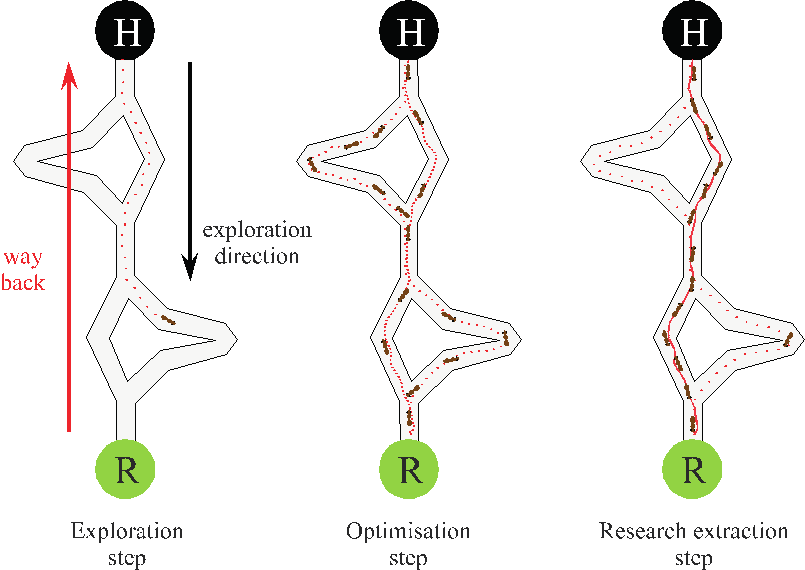
\includegraphics[width=0.75\textwidth,keepaspectratio]{Images/aco.jpg}
                \caption{Ants finding the optimal path from the start to the finish in a simple graph.}
                \label{fig:ant}
            \end{figure}            
    
            The foundation of ACO is built with pheromone trails, ant behavior, local search and construction, and pheromone updates including evaporation over time. Pheromone trails represent the collective memory of the ant colony and guide the exploration of the solution space. Initially, pheromone trails are uniformly distributed. As ants traverse paths, they deposit pheromones, with the quantity proportional to the quality of the solution found. Pheromone evaporation ensures adaptability and prevents premature convergence. Ants probabilistically select paths based on a combination of pheromone information and heuristic knowledge. The pheromone trail intensifies the attractiveness of paths with higher pheromone concentrations, while heuristic information guides exploration towards promising regions of the solution space. Ants may employ stochastic decision rules such as probabilistic selection of paths using some random generation to encourage exploration and not just blindly following the ants that came before. Ants construct solutions incrementally by selecting and appending components of partial solutions. Some variants of ACO use a simple local search mechanisms, such as 2-opt or 3-opt, to try and improve on the found solution, but this step adds considerable runtime complexity and isn't necessary for achieving solutions of sufficient quality. After each iteration, pheromone trails are updated to reflect the quality of constructed solutions. Pheromone evaporation will ensure the decay of pheromone concentrations over time, preventing stagnation and promoting exploration. Additionally, pheromone reinforcement is applied to paths traversed by high-quality solutions, intensifying their attractiveness to subsequent ants.
            
            ACO has been widely applied to solve the TSP, with numerous variants and extensions developed over the years. These approaches have demonstrated the effectiveness of ACO in finding high-quality solutions to TSP instances, often outperforming traditional heuristic methods. ACO often produces high-quality solutions by effectively exploring diverse regions of the solution space through pheromone communication. ACO exhibits strong convergence properties and, as a particle swarm algorithm, is highly parallelizable and scalable. This makes ACO suitable for large problems where other heuristic algorithms start to struggle.

            \subsubsection{Formal Mathematical Definition}
            ACO operates by iteratively constructing candidate solutions using a population of virtual ants. Each ant probabilistically selects paths based on the pheromone trails deposited by previous ants. As ants traverse paths, they deposit pheromones, which influence the decisions of subsequent ants. Over time, the concentration of pheromones on promising paths increases, guiding the exploration towards better solutions.
            
            The mathematical model for ACO is given by the following four equations:
            {\Large
            \begin{align}
                p_{i, j}^{k} &= \left\{
                \begin{array}{ll}
                    \frac{\left[ \tau_{i,j} \right]^{\alpha} \cdot \left[ \eta_{i, j} \right]^{\beta}}
                    {\sum_{s\in\text{allowed}_{k}}\left[\tau_{i, s}\right]^{\alpha} \cdot \left[\eta_{i, s}\right]^{\beta}} & j\in \text{allowed}_{k}\\
                    0 & \text{otherwise} \\
                \end{array} 
                \right. \\
                \tau_{i, j}\left(t+1\right) &= \rho \cdot \tau_{i, j}\left(t\right) + \Delta\tau_{i, j}\\
                \Delta\tau_{i, j} &= \sum_{k=1}^{l}\Delta\tau_{i, j}^{j}\\
                \Delta\tau_{i, j}^{k} &= \left\{
                    \begin{array}{ll}
                        \frac{Q}{L_k} & \text{if ant $k$ travels on edge $\{i, j\}$} \\
                        0 & \text{otherwise}
                    \end{array}
                \right.
            \end{align}
            }
            where the following parameters are used: 
            \begin{itemize}
                \item $p_{i,j}^k$ is the probability that ant $k$ will traverse the edge from city $i$ to city $j$.
                \item $\tau_{i, j}$ is the pheromone intensity along edge $\{i, j\}$
                \item $\eta_{i, j}$ is the edge weight along edge $\{i, j\}$
                \item $\alpha$ is a constant to regulate the influence of $\tau$
                \item $\beta$ is a constant to regulate the influence of $\eta$
                \item $s$ is some city/node that has not yet been visited by ant $k$
                \item $\rho \in \left[0, 1\right]$ to regulate pheromone decay
                \item $\Delta\tau_{i,j}$ is the amount of pheromone to increase along edge $\{i, j\}$
                \item $Q$ is a constant to regulate the influence of ant fitness on pheromone increase
                \item $L_k$ is the total length of ant $k$'s tour
            \end{itemize}
            The following pseudocode is a general implementation of Ant Colony Optimization that does not include parallelization or our specific implementation, yet is simply stated to highlight the important aspects of the algorithm.
            \begin{algorithm}[!h]
                \DontPrintSemicolon
                \caption{Ant Colony Optimization}
                \label{alg:aco}
                \KwResult{}
            
                Initialize $pheromone\_trails$\;
                Initialize parameters\;
                $best\_solution\gets\{\}$\;
                \While{Stopping criteria is not met}
                {
                    \tcc{Construct solutions for each ant}
                    \ForEach{$ant\in all\_ants$}
                    {
                        Initialize ant memory\;
                        $visited\_set\gets\{\}$\;
                        Randomly select a $start\_node$\;
                        Add $start\_node$ to $visited\_set$\;
            
                        \While{$||visited\_set|| < all\_nodes$}
                        {
                            Probabilistically select next component in solution based on pheromone trails and heuristic information\;
                            Update $visited\_set$\;
                            Update pheromone trails\;
                        }
                    
                        Apply local search to ant memory\;
                        \If{solution is better than $best\_solution$}
                        {
                            $best\_solution\gets$ solution\;
                        }
                    
                        Update pheromone trails based on solution quality\;
                    }
                    Evaporate pheromone trails\;
                }
                
                \Return{$best\_solution$}
            \end{algorithm}

        
        \subsection{Setup of CUDA Development Environment}
            The parallelizability of an algorithm depends on the presence of some tasks, particularly ones that consume a large amount of computational time, that can operate independently; meaning every task to be executed in parallel must not immediately depend on the results of a previous run of the same task and must not alter any shared space in memory. Many operating systems do not use Concurrent Read, Concurrent Write (CRCW) Parallel Random Access Memory (PRAM) architecture, and may allow for multiple threads to concurrently read from memory, but not alter it concurrently. CUDA's architecture will allow for concurrent writing, and requires careful management of memory addresses to ensure that no accidental write overlap occurs.
            
            CUDA was leveraged as the programming model and C/C++ as the programming languages. This project utilized NVIDIA's CUDA Toolkit and libraries for parallelizing computations and managing memory transfers between the CPU and GPU. An implementation of a parallel ACO algorithm was developed specifically for GPU architectures using CUDA. This algorithm adheres to the fundamental principles of ACO, encompassing ant population initialization, pheromone updating, and solution construction. Leveraging the parallelism inherent in GPUs, multiple arrays were employed to represent essential data structures such as the pheromone matrix and adjacency matrix. Additionally, arrays were used to track various statuses of individual ants, including their best tour found, current tour, and visited cities. These arrays were meticulously allocated with sufficient space to enable concurrent writing by each ant. 
            
            To ensure thread safety and maximize parallelization efficiency, a CRCW PRAM methodology was adopted, thereby mitigating data race conditions. By using the unique thread and block IDs, each ant thread knows precisely where it is permitted to write within the shared memory blocks. Furthermore, the parallel algorithm employs multiple kernel calls per iteration: one for ant movement, another for pheromone evaporation, and a third for pheromone matrix updates. Each thread in the ant movement kernel corresponds to an individual ant, while each thread in the pheromone matrix evaporation kernel handles one edge of the matrix. Finally, each ant is responsible for updating all edges in the pheromone matrix that it traverses, ensuring comprehensive pheromone update coverage. This allows a fully parallelized ACO algorithm. When given a large number of ants, the GPU can be flooded to operate as close to maximum capacity as possible, utilizing as much of the hardware to tackle large problem instances. Overall, this implementation prioritized efficiency, scalability, and thread safety to enable the successful execution of the parallel ACO algorithm on GPU platforms.
        
        \subsection{Parallelization of Ant Colony Optimization Tasks}
            \subsubsection{Ant Run Independence}
            Each ant uses two important pieces of information for create a tour: the adjacency matrix and pheromone matrix. These two data structures all the ant to traverse the problem landscape for the creation of tours. Because these two structures are not being actively changed as the ants complete their tours, the ant's input independence is maintained. As ants travel, they store their tours in a globally available ant history matrix. This structure is being manipulated by multiple ants at a time (as is made possible with CRCW PRAM architecture). However, since each ant is has a unique identifier which is extracted from its thread and block identifiers, and the structure is large enough to accommodate the number of ants being sent, each ant will only change a row of the history matrix according to its unique identifier. This prevents any overlap, and maintains the output independence of the process.
            
            \subsubsection{Pheromone Matrix Updating Independence}
            For the updating of the pheromone matrix, the ant run history, ant tour distance, and the pheromone matrix are all required for the updating of the pheromone matrix. Unfortunately, since the output is also included in the input, as ant histories are being iterated through in parallel, there is a chance that write overlap may occur, interfering with the independence of the process. To address this, the CUDA runtime library allows for atomic locking locations in memory so that once a thread locks the location in memory, other threads that attempt to access the same location must queue until the write is complete. However, since the likelihood this will occur is marginal, and threads will most likely be attempting to update separate locations in memory at any given point in time, the independence requirement will be upheld most of the time, which means this process can be executed in parallel. 

    \section{Experimental Setup}
    The experimental suite consisted of running two different experiments to evaluate the performance of the parallel Ant Colony Optimization algorithm for solving the TSP using CUDA. The first experiment was performed on a system equipped with a NVIDIA RXT 3080ti GPU. A standard benchmark dataset for TSP instances was used, detailed below, consisting of instances between 14 and 100 cities. This experiment suite was a demonstration of the algorithm's abilities to run on smaller problem instances before conducting a large scale test. The second experiment was performed over the course of 12 hours, utilizing 40 NVIDIA RXT 4090 GPUs that each operated on a range of large scale problems. These problems varied in size between 100 and 3038 cities. Each computer's results were stored in a shared network drive, simulating setups commonly found in loosely distributed clusters of GPUs.   
    
    The benchmark datasets used in this experiment include both symmetric and asymmetric problem instances found at \href{http://comopt.ifi.uni-heidelberg.de/software/TSPLIB95/}{TSPLIB}. There were 27 asymmetric TSP instances, and 112 symmetric instances. All of the problems included their optimal solution, so a direct comparison between the ACO-found solutions and the known optimal was possible. 
    
    The performance of this algorithm was based on the quality of solutions obtained and computational efficiency. The primary evaluation metric used was the percentage deviation from the global optimal solution. Additionally, the runtime of the algorithm was measured for each instance to assess its scalability and efficiency.
    
    To find the optimal set of hyperparameters in this model, multiple small experiments were run using different configurations, varying parameters such as the number of ants, pheromone update rules, and CUDA thread block size. It was experimentally determined that the following parameters provided sufficient results on large scale problems without sacrificing runtime:
    \begin{table}[h]
    \centering
    \label{tab:hyperparameters}
    \begin{tabular}{|l|c|}
        \hline
        Threads per Block & 512 \\
        \hline
        Number of Blocks & 80 \\
        \hline
        Pheromone Importance ($\alpha$) & 1.0\\
        \hline
        Heuristic Importance ($\beta$) & 2.0\\
        \hline
        Evaporation Rate ($\rho$) & 0.4\\
        \hline
        Pheromone Deposit & 100.0\\
        \hline
        Number of Iterations & 100\\
         \hline
    \end{tabular}
    \caption{Model hyperparameters}
    \end{table}
    \\
     The hyperparameters of the model were carefully determined in consideration of both the hardware used and the nature of the problem. The parameters that controlled the number of threads per block and number of blocks were determined by the hardware used. In GPU programming, it is better to flood the GPU with as many threads as possible, so that all of the hardware is utilized properly. On the RTX 4090, there are 16,384 CUDA cores. To flood the GPU, there would need to be at least 16,384 threads. The maximum threads each block supports is 1024, so there would need 16 blocks at least. However, due to the memory optimization of the GPU, it's better to distribute many threads over many blocks, so the decision was made to use 512 threads per block and 80 blocks. This provided a total of 40,960 threads, which more than floods the GPU. Each ant was given 1 thread, so there were also 40,960 ants. This was done to ensure that the GPU is fully utilized. The parameters that determined the behavior of the ants was determined initially from literature recommended values, then from experimental tweaking. The literature recommended values for $\alpha, \beta, \text{and} \rho$ are $1.0, 4.0, 0.5$ respectively. In the probability equation, the pheromone importance is raised to $\alpha$ and the heuristic distance is raised to $\beta$, so these parameters indicate that heuristic information was much more influential than pheromone information. This ensures that the ants don't follow a really strong, albeit bad, solution just because other ants have walked on that path many times before. The standard evaporation rate is $0.5$, indicating that 50\% of pheromones disappear after each iteration. However, when experiments were being run, it was noticed that occasionally the right pheromone trails would evaporate too quickly, leading to the ants walking worse paths each successive iteration and losing the higher quality solutions. Thus, the percentage of evaporation was lowered to ensure that solutions didn't evaporate before they could be properly established. The constant for pheromone deposit was also determined by literature. The recommended value is $1.0$, but because this algorithm used thousands of ants, this parameter was scaled to decrease the likelihood that any rounding errors would be encountered. Considering how some solutions were in the tens or hundreds of thousands unit distance, rounding errors could have been possible. 
     
     Each problem instance was repeated 30 times to ensure statistical significance and reduce variability. A sample size of thirty independent runs increases the confidence interval of the sample data set enough to claim a valid representation of the population \cite{clt2008}. This number also warrants assertions of statistical significance.
    
    \section{Performance Metrics and Benchmarking Results}
        The results of this experiment demonstrates the effectiveness of the parallel ACO algorithm in solving the TSP instances. Not all large problem instances were able to finish computing in the provided experiment time of 12 hours, so those results are excluded here. The Relative Percent Difference (RPD) of the best found solution in each test run was compared to the known best solution for that problem instance. On average, the parallel ACO algorithm achieved an RPD of 7.4327\% from the global optimal solution across all test cases, ranging from instances with 14 to 3038 cities. There was a standard deviation of 6.19\% between all test cases. The global optimal solution was found in 9 of the problem instances, the largest of which was a 180 city instance. 13 of the instances were solved within 1\% of the global optimal, 33 instances were within 5\% of the global optimal, and 52 were within 10\%. The worst RPD of all problem instances was the 3038 city instance, where solutions at worst 20.5035\% away from the global known best were found. It can be seen in Figure \ref{fig:rpd} the graph of the average RPD of all 30 test runs compared to the best RPD out of those 30 runs for each problem tested. 

        The quality of solutions obtained by this algorithm was evaluated by comparing them to known optimal solutions for each TSP instance. In Figure \ref{fig:rpd} it is shown that every problem less than 500 cities in size was solved within 10\% of the optimal. The performance is worse in the problems above 500 cities; however, the best solutions found were within 20\% of the global optimum except for the 3038 city problem instance. Further refinement of the algorithm, including implementing some of the variant ACO algorithms, specifically the AS-LBT, should show improvements upon these already good results. 

        \begin{figure}[h]
            \centering
            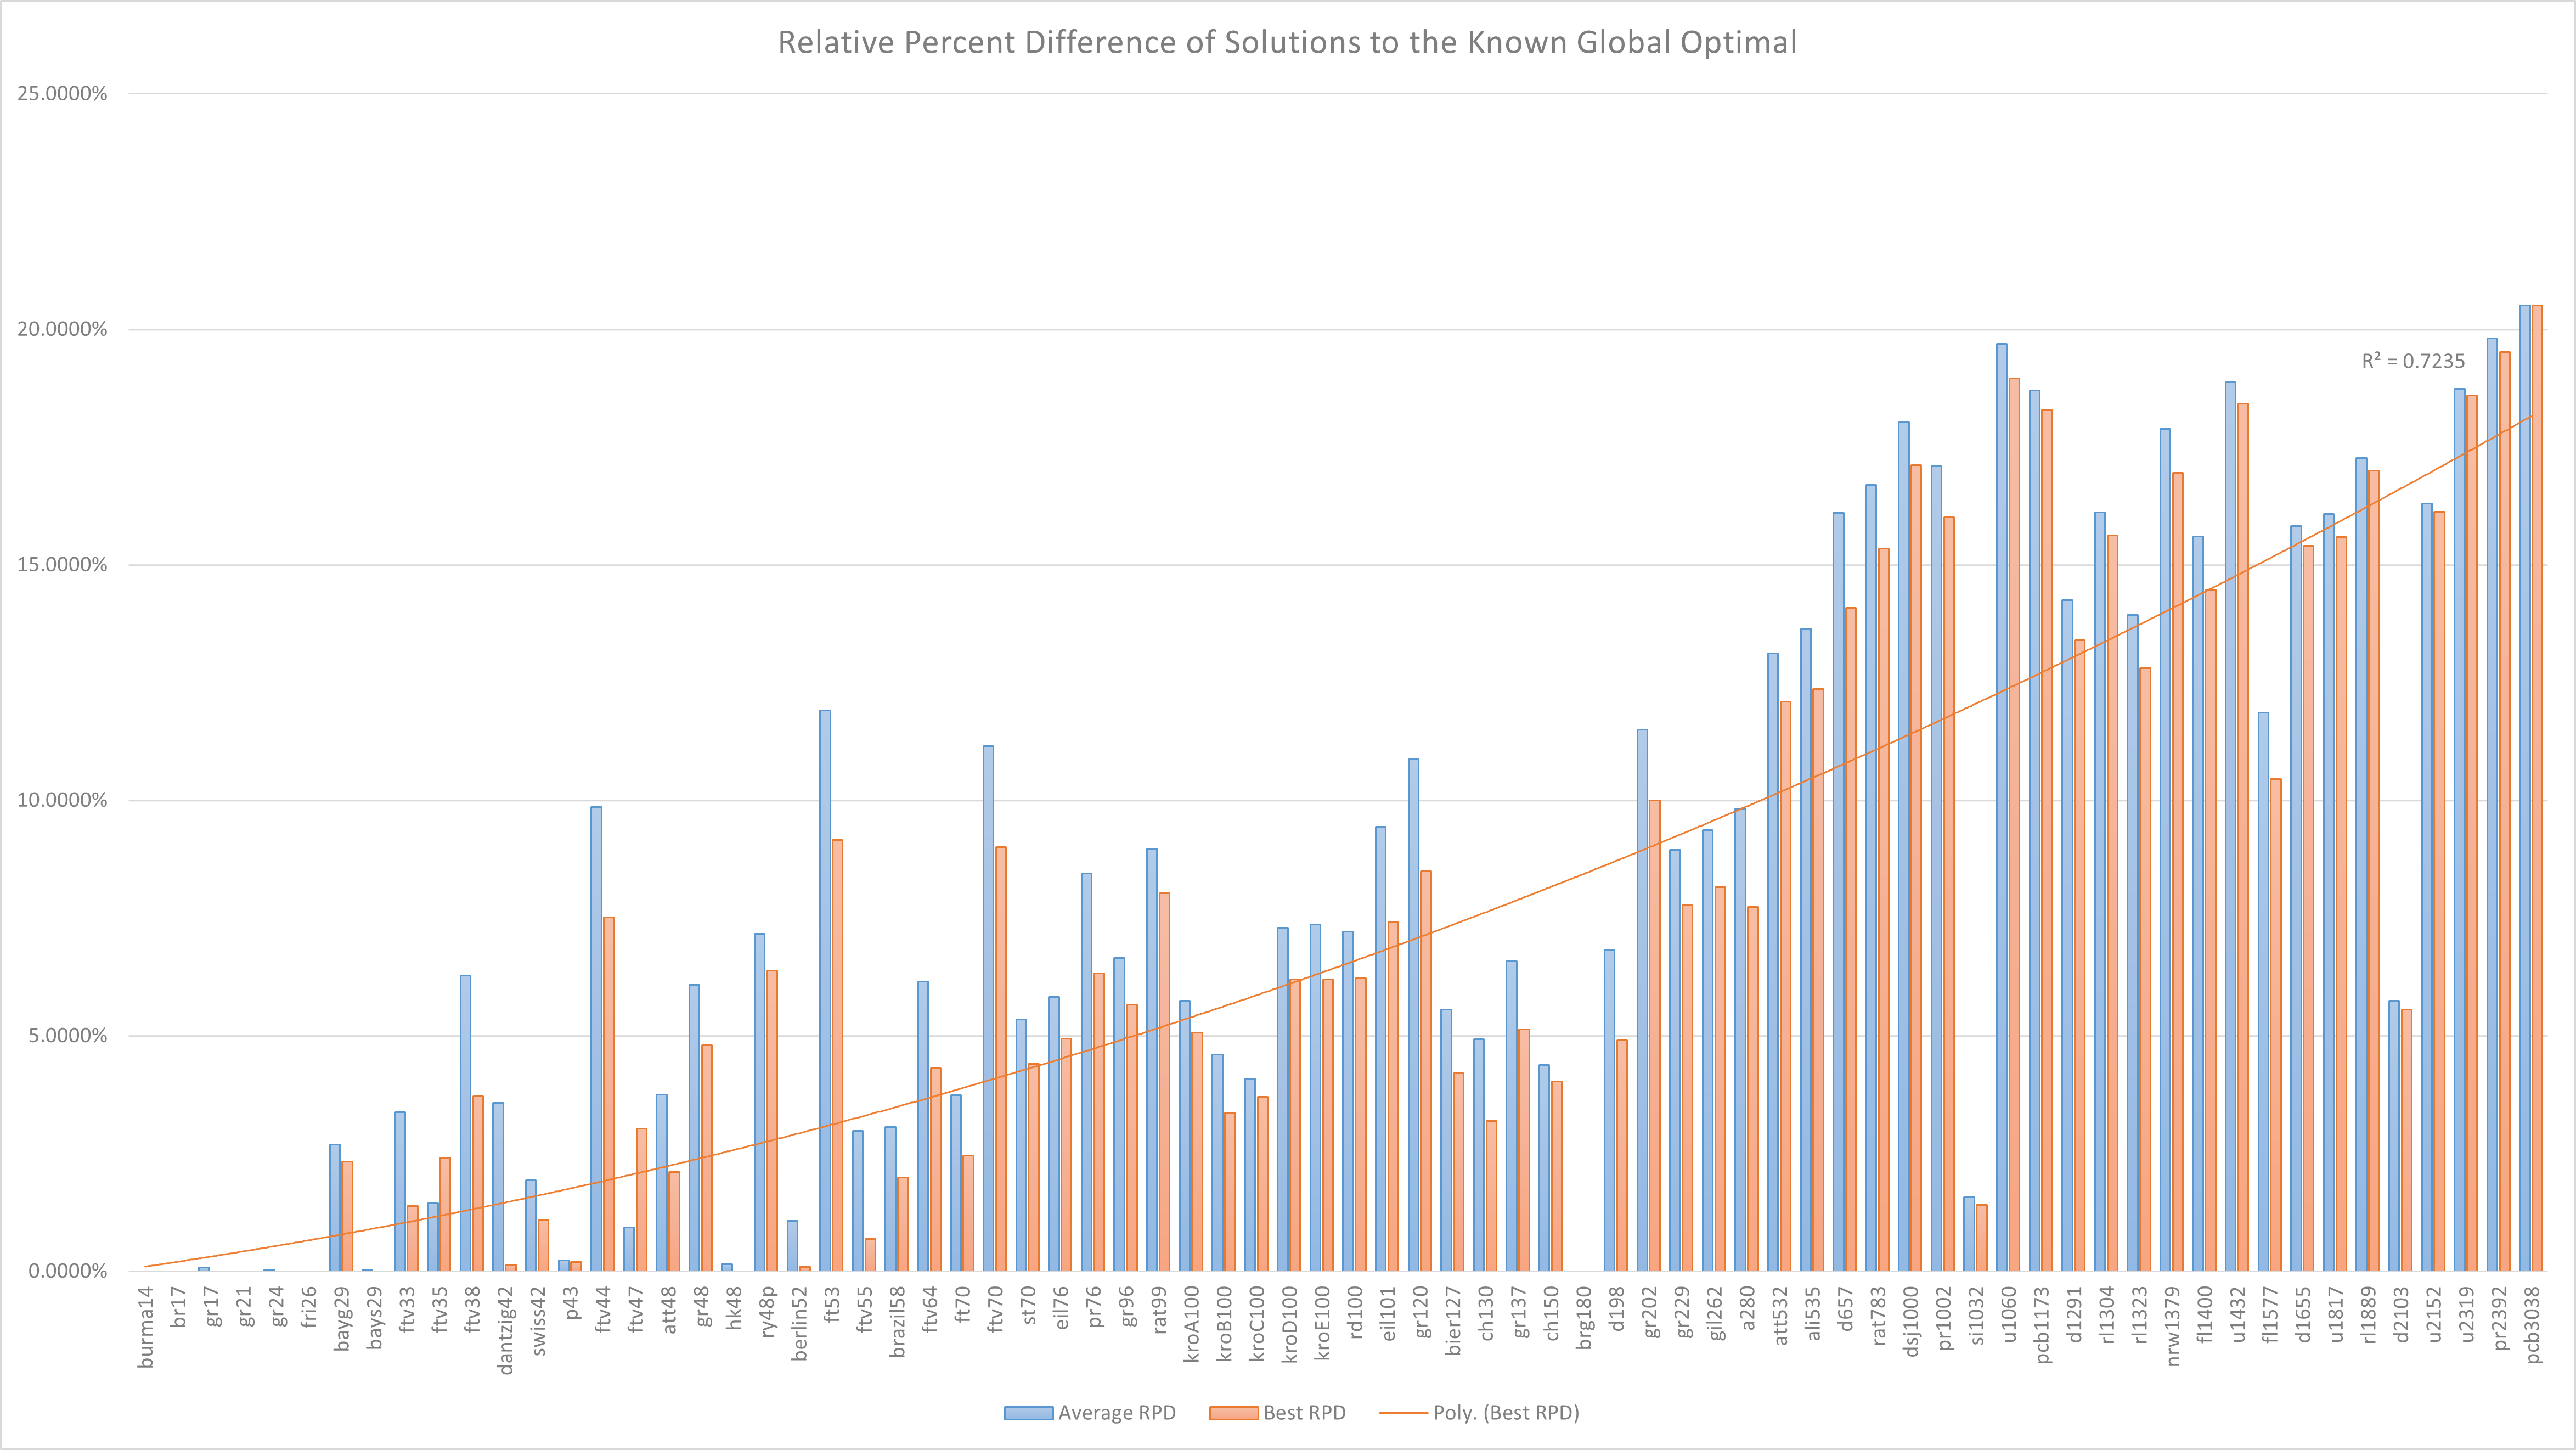
\includegraphics[width=0.9\textwidth,keepaspectratio]{Images/PRD}
            \caption{Graph of the RPD of the average solution generated compared to the best solution found for all fully tested problem instances.}
            \label{fig:rpd}
        \end{figure}
        \newpage
        
        \subsection{Speed-Up Analysis and Performance Evaluation}
            In addition to solution quality, the runtime was measured for each TSP instance. By analyzing the Ant Colony Optimization algorithm, it is known that the runtime of ACO is exponential in terms of problem size, so it is not unexpected to see that the runtimes increased exponentially as problem sizes grew, as shown in Figure \ref{fig:time}. Note that this figure's y-axis is logarithmic scaled. It can clearly be seen that an exponential trend with a strong correlation constant proves that the runtime increased exponentially with respect to problem size. 

            \begin{figure}[h!]
                \centering
                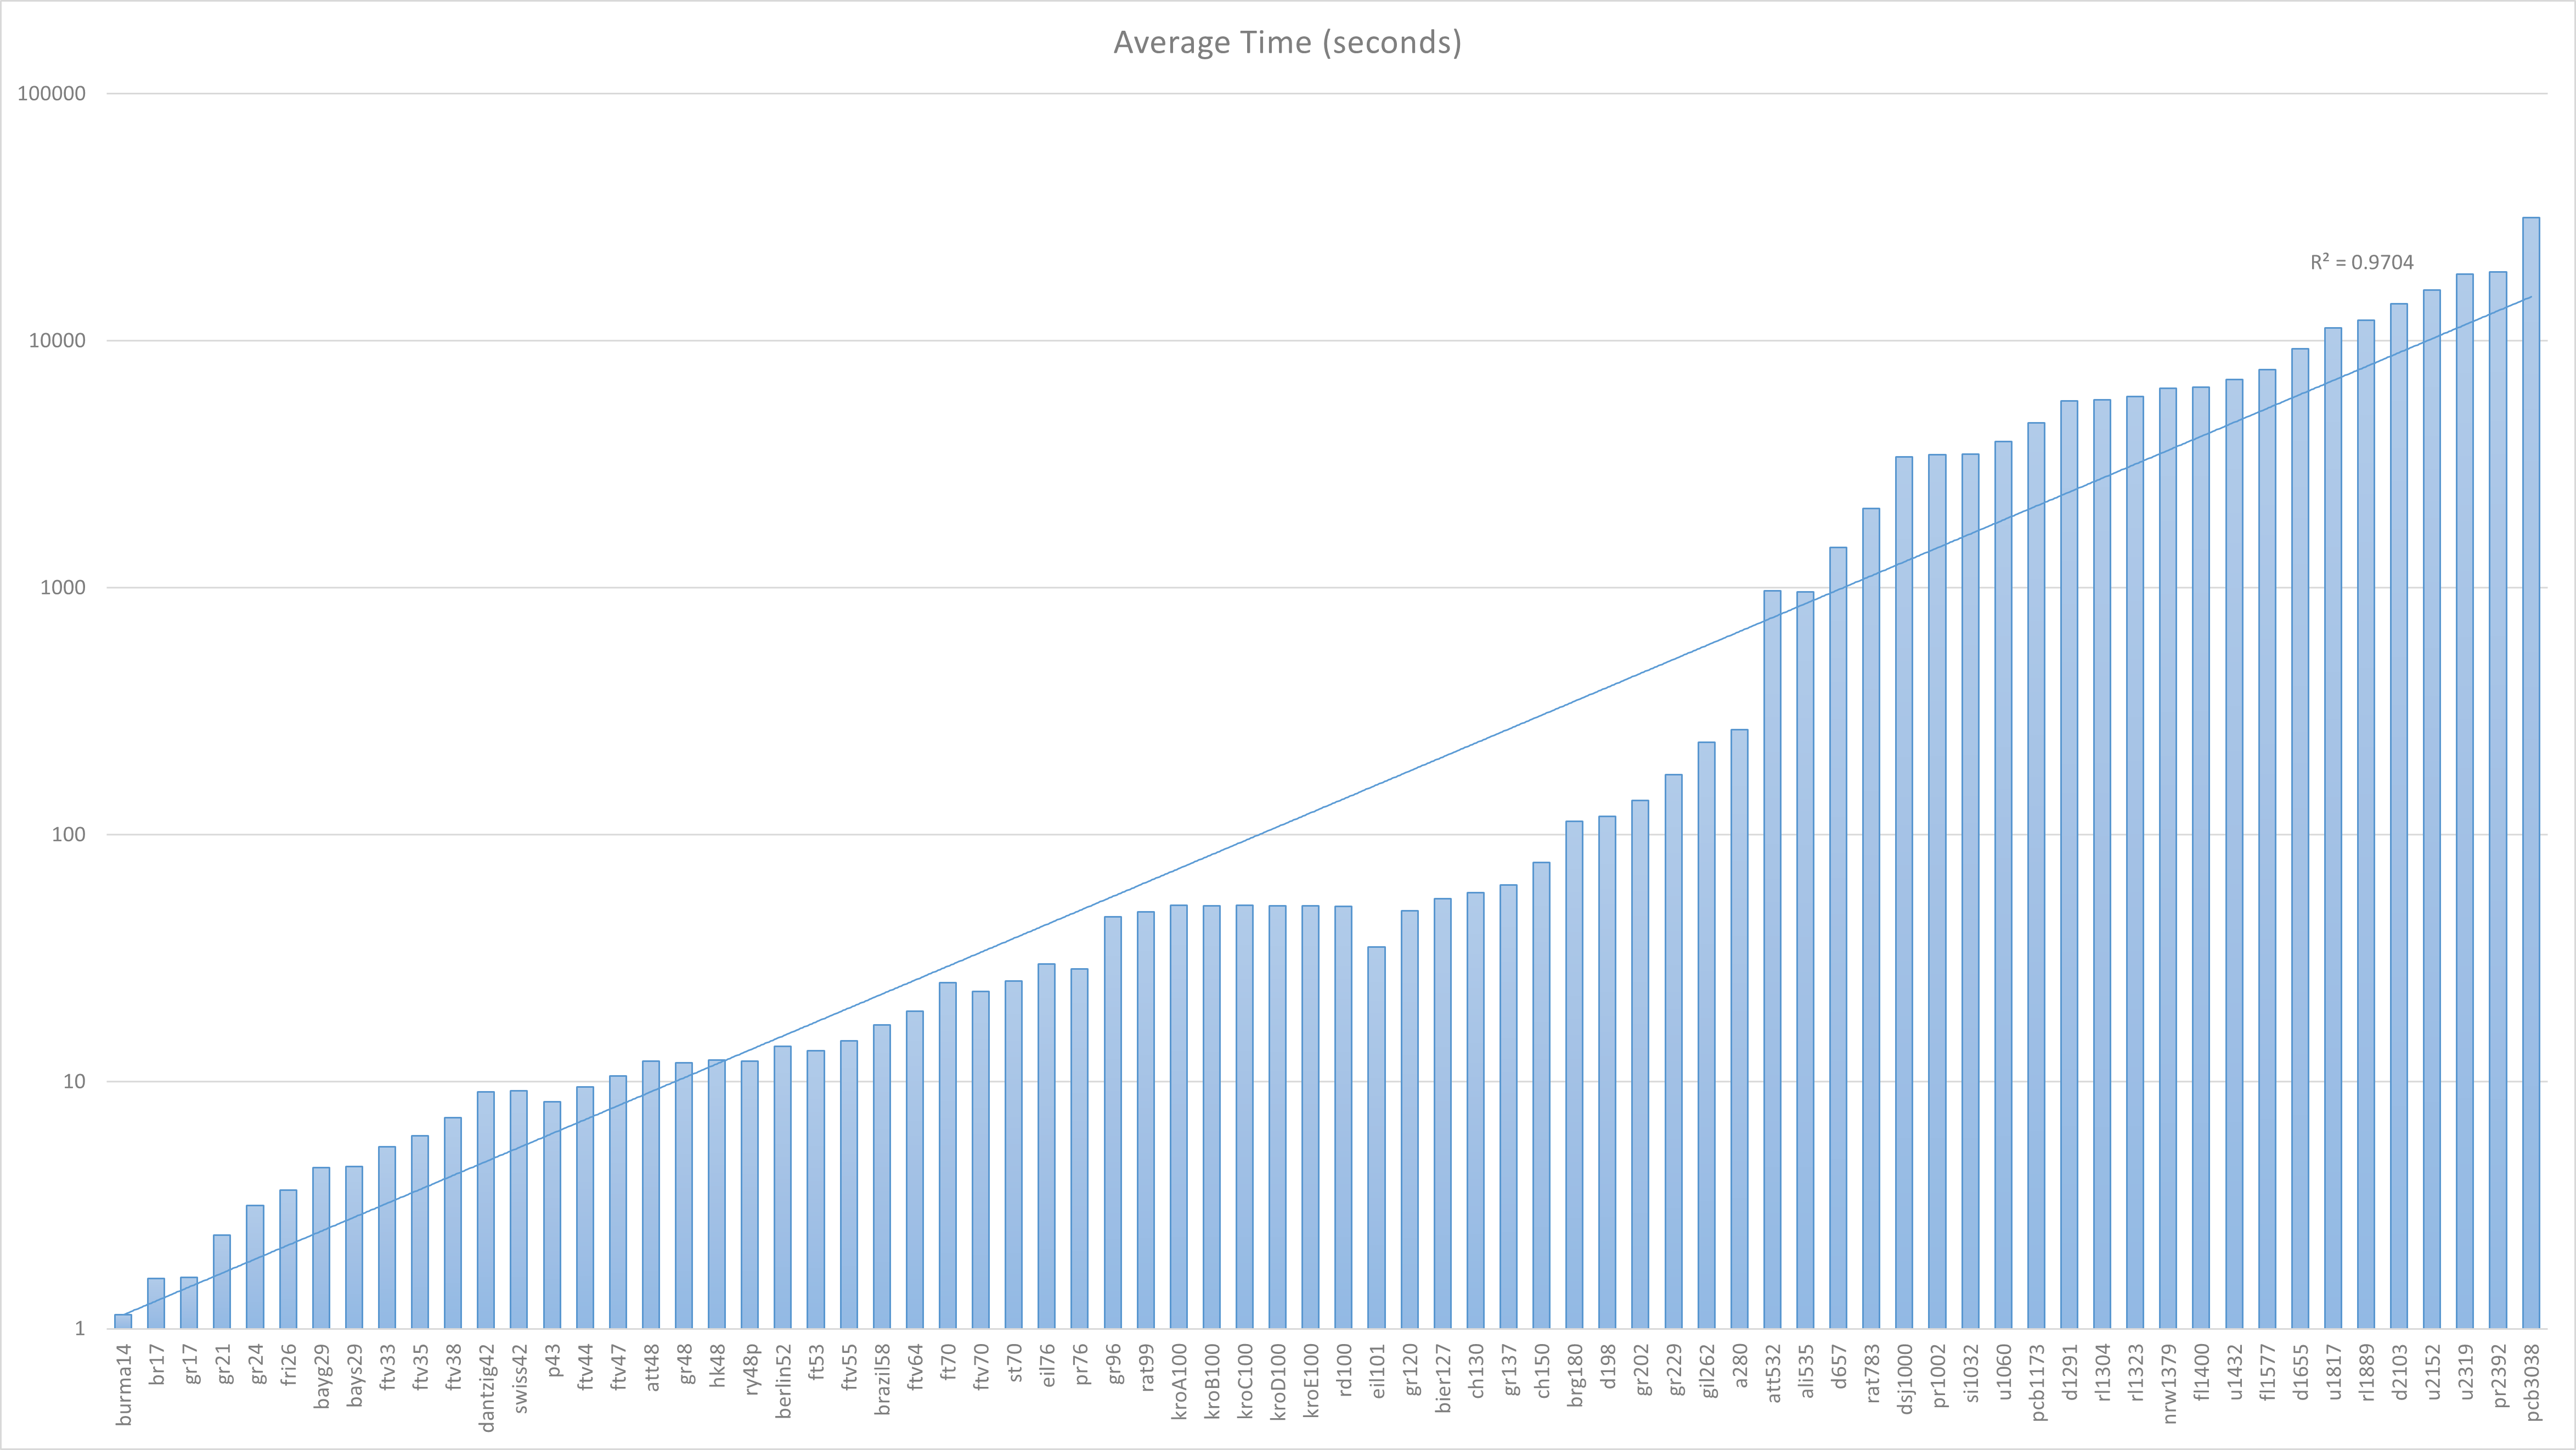
\includegraphics[width=0.9\textwidth,keepaspectratio]{Images/Time}
                \caption{Graph of the average time taken to compute a solution for each problem instance. Note that the y-axis is logarithmic scaled, not linear.}
                \label{fig:time}
            \end{figure}
            \newpage
            

        \subsection{Resource Utilization and Efficiency Metrics}
            The nature of CUDA enables GPU devices to require the copying of memory from the host system to the device. Because this process can take up a substantial amount of computational time, reducing the amount of data transfers between the host and device is critical to maintaining runtime efficiency. To achieve this, memory allocation is split across the host and device.

            \subsubsection{Host Memory}
            Memory maintained by the host system might include the following:
            
            \begin{itemize}
                \item \textbf{Adjacency Matrix}, either read or computed from data available on the host system.
                \item \textbf{Best Distance per Iteration}, a desired piece of information to record how the quality is improving between iterations.
                \item \textbf{Best Tour per Iteration}, the tour which achieves the Best Distance per Iteration.
                \item Any other recorded data relating to how the algorithm is performing.
            \end{itemize}
            
            Essentially, host memory is dedicated to the problem landscape being navigated, although it does not require being permanently stored by the host, along with data to be recorded periodically by the performance of the algorithm. Unfortunately, as data is recorded, it will require some data transfer between the host and device to get this kind of information, so keeping the desired data to a minimum would improve the runtime of the algorithm.
            
            \subsubsection{Device Memory}
            Memory maintained by the device is all data that is essential for all processes being run in parallel. Keeping this memory to a minimum will ensure that the problem can scale to larger sizes. These memory points include the following:
            
            \begin{itemize}
                \item \textbf{Adjacency Matrix}, the problem landscape to be navigated so ants can consider the edge weight between points.
                \item \textbf{Pheromone Matrix}, the sway of the collective on an ants decision making process.
                \item \textbf{Ant Run History}, the history of an ant's route through the problem landscape. This is updated every time an ant makes a decision, and is essential for the recording of an optimal tour and updating the pheromone matrix.
                \item \textbf{Visited Cities}, a simple, low memory, structure for ants to ''remember" where they have been so they don't mistakenly return to a city they have been before. This structure is separated by Run History to reduce the runtime for checking if an ant has been to a city before.
                \item \textbf{Distance History}, the total of an ant's tour so far. After all ants complete their runs, this distance history will represent the tour length of the tour stored in Ant Run History.
            \end{itemize}
            
            A breakdown of the size of these structures can be seen in Table 1, where $n$ is the number of cities and $k$ is the number of ants
            
            \begin{table}[]
            \centering
            \caption{Representation of the size of the memory structures on the parallel device.}
            \begin{tabular}{|l|l|l|l|l|}
            \hline
            Property         & Data Type                & Data Type Size           & Dimensions               & Device Memory   \\\hline
            Adjacency Matrix & Double                   & 8B                       & $n \cdot n = n2$               & $8(n \cdot n) = 8n^2$B  \\\hline
            Pheromone Matrix & Double                   & 8B                       & $n \cdot n = n^2$               & $8(n \cdot n) = 8n^2$B  \\\hline
            Ant Run History  & Integer                  & 4B                       & $n \cdot k = nk$               & $4(n \cdot k) = 4nk$B  \\\hline
            Visited Cities   & Boolean                  & 1B                       & $n \cdot k = nk$               & $n \cdot k = nk$B      \\\hline
            Distance History & Double                   & 8B                       & $k$                        & $8k$B              \\\hline
            \textbf{Total}   & \cellcolor[HTML]{9E9E9E} & \cellcolor[HTML]{9E9E9E} & \cellcolor[HTML]{9E9E9E} & $16n^2 + 5nk + 8k$Bs \\\hline
            \end{tabular}
            \end{table}

            \newpage
    \section{Impact of Problem Size and Complexity}

        \subsection{Scaling Analysis and Computational Efficiency}
            \noindent Some of the problems were large enough that they didn't finish computing, meaning that this algorithm wasn't feasibly scalable for very large problem instances. There are many reasons this could be the case, and these reasons are discussed later. However, looking at Figure \ref{fig:aco-runtime}, it is shown that the runtime of ACO decreases exponentially as more threads are introduced \cite{borisenko2019}. This shows that even though some problems were infeasibly large for the current implementation of ACO, running this without using the CUDA framework distributed over 40 16,384 core RTX 4090 cards, there would have been a much longer runtime. As such, the comparison should instead be focusing on the height of each of the bars in Figure \ref{fig:time}. In the worst case, this algorithm ran in the range of $10^5$ seconds. Granted, that is $\sim8.75$ hours, but when considering the size of the search space of $3038! \approx 7.168091361\cdot10^{9262}$, finding a solution within 20\% of the global optimal in only $\sim8.75$ is a huge feat. By the estimates in Figure \ref{fig:aco-runtime}, a single core with the same hyperparameters would have had well over $400\times$ the runtime to generate the same solution. 
            
            \begin{figure}[h!]
                \centering
                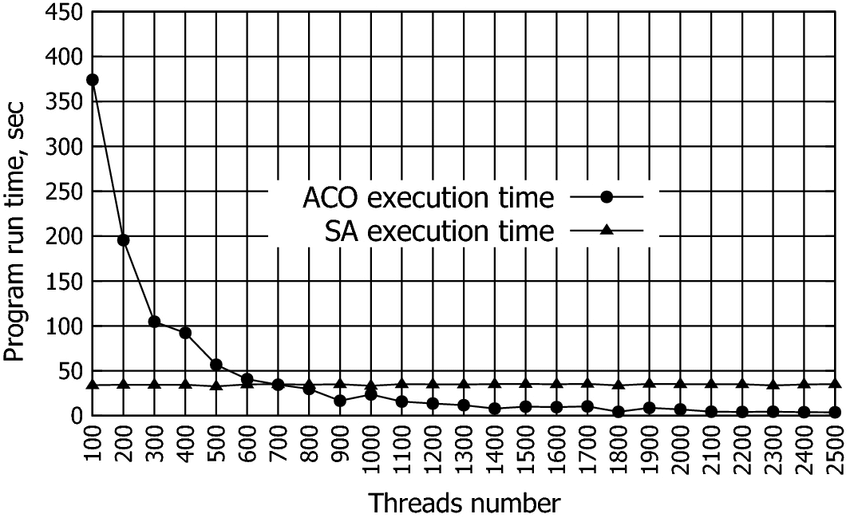
\includegraphics[width=0.65\textwidth,keepaspectratio]{Images/Run-time-of-ACO}
                \caption{Figure showing the runtime of ACO decreasing exponentially as new threads are introduced.}
                \label{fig:aco-runtime}
            \end{figure}
            \noindent However, the time complexity and comparison can be broken down further using the data gathered. For the 3038 city instance in particular, this implementation in parallel visited $40,960 \cdot 3038 = 12,443,648,000$ cities per iteration, or $1.24$ trillion cities per solution generated. One solution took on average $31,538$ seconds to compute, meaning that the ants in that problem visited on average $39,456,047$ cities per second. Because each GPU has $16,384$ cores, on average each core computed the visitation to $2,408$ cities per second. To put this all in perspective, if there was a CPU with the exact same clock speed and general performance, but only one core, that core would have to run for a total of $16.385$ years to compute 1 solution. This is substantially more than $400\times$ runtime required, and shows how much performance gain CUDA allowed.  
            
            A fixed number of ants was used for all our problem instances. With 512 threads per block and 80 blocks, there were 40,960 ants per problem as previously discussed. While this worked to generate high quality results throughout all of our problem instances, many of the smaller instances would generate a good answer within 2 to 5 iterations. The large number of ants was able to overwhelm the search space, leading to finding the optimal or close to the optimal purely by chance very quickly. This would lead to a lot of iterations where the algorithm wasn't improving, and the computational power was effectively wasted. To mitigate this problem, a variable number of ants could be used. The number of ants could be partially determined by the problem size, so that small problems have less ants whereas large problems have more ants. This way, the algorithm can dynamically adjust to the size of the solution space so that the resources can be utilized fully. This could reduce the times shown in Figure \ref{fig:time}, further improving the algorithm.


    \section{Analysis and Interpretation of Findings}
        The utilization of CUDA parallel computing enabled the leveraging of the computational power of GPUs, resulting in scalable and efficient TSP solving. By parallelizing critical algorithmic components and optimizing memory access patterns, this algorithm significantly reduced the computational time required to find high-quality solutions for large-scale instances of the TSP. The success of this parallel ACO algorithm highlights the potential of GPU-accelerated computing in addressing real-world optimization challenges.
        
        Further optimization and refinement of the parallel ACO algorithm could lead to even better solution quality and computational efficiency. One of the popular variants of the ACO is the Ant System - Local Best Tour (AS-LBT). This variant can substantially improve the quality of the solutions found\cite{White03}. The ACO algorithm quickly converged to a high quality solution within the first 5 to 10 iterations, and then from iteration 10 to 100, the algorithm would stagnate and hover around the same solution. Determining a dynamic early stopping criteria could reduce the computational time for when solutions start to stagnate. Implementing any of the variants to ACO could also further improve the solution quality. In AS-LBT, no additional runtime complexity is added for significant gains on the results of the algorithm\cite{White03}.
        
        Furthermore, double precision values were used to store the pheromones, adjacency matrix, and the ant solutions. The GPUs used have significantly better performance when using float values instead of double values. The theoretical performance of an RTX 4090 when using float values is 82.58 TeraFLOPS (Float Operations Per Second), whereas using double values reduces the performance significantly to 1,290 GigaFLOPS. This information was not known before the experiments were run, and is a glaring performance hit, especially considering the extra precision with double values would not improve the quality of the solutions. The problem instances used in this experiment were all provided in floating point precision, so using doubles unnecessarily increased the precision of this model without gaining any significant information and losing huge portions of performance. This was an oversight when building the model. Future work can be done to change the code and compare the time speedups between double and float performance on the GPUs.
        

\chapter{Discussion and Conclusions}


    \section{Implications of CUDA for Combinatorial Optimization}
    CUDA offers an accessible API for programmers to create or port exiting applications that make use of GPU resources for accelerated computations. While not every application will benefit from this acceleration, those that do are exposed to highly scalable possibilities on a hardware platform that sees massive improvments on a regular basis.

        \subsection{Advantages and Limitations of GPU Acceleration}
        While GPU acceleration offers the capability of processing many threads at a time, the lower execution frequency of each core compared to even older CPUs makes GPU acceleration unsuitable for applications that do not require such a high number of parallel components, and might be better suited running on a CPU cluster rather than a GPU cluster. However, combinatorial optimization problems require a large number of explorations due to their immense solution space, making access to an increased number of concurrently executing threads ideal.

        In the case of Ant Colony Optimization (ACO) for solving TSP, as covered in the previous chapter, each ant attempted to produce a feasible solution according to the ACO algorithm. Therefore, increasing the number of ants that are looking for a solution is paramount for improving solution quality. Conversely, an application interface dependent on user input, would not require such high parallelism, since much of the time running a process may be spent waiting for the user to interact with the program. Because of this, a single core of a CPU may be sufficient for a user application. And if multiple users are interacting with the same application at the same time, a second core of any multi-core CPU would similarly be sufficient.

        GPU acceleration may also prove unsuitable for processes which require a large amount of memory per thread. Ideally, algorithms can be modified so that tasks can be split up evenly among threads so as to speed up a process on a smaller portion of memory; but in instances where this is impossible, GPU acceleration may not provide sufficient speedups.

        \subsection{Practical Applications and Future Prospects} 
        GPU acceleration to combinatorial optimization offers solutions to otherwise infeasible problems; especially as the number of realistic constraints increases. Although the solution space decreases on problems as the number of constraints increase, the time it takes to find a single feasible solution increases. Using GPU acceleration, more feasible solutions can be calculated in parallel, making better answers to increasingly complex problems more attainable.

        The results to such solutions may manifest as more efficient travel or deliver routes which may provide a reduction in travel and devilry times as well as a reduction in greenhouse gas emissions and energy consumption. Perhaps optimization algorithms may provide better insight when designing civil infrastructure, leading to a more efficient use of natural resources and public spending. 

        \subsection{Beyond Combinatorial Optimization}
        As the advent of Artificial Intelligence grows, training these models requires access to large data sets and computers powerful enough to process them. GPUs have offered the solution for the creation of systems capable of meeting such training requirements\cite{GPU_ACCELERATION_OF_AI}.

        Another application of these Artificial Intelligence systems outside the realm of optimization. Predictive algorithms, while presenting an ethical dilemma when applied to predicting human behavior (such as COMPAS\cite{COMPAS_REVIEW} and the infamous predictions of Target Retailers\cite{HOW_COMPANIES_LEARN_YOUR_SECRETS}) and vulnerability to bias\cite{AI_EXPLAINABILITY}, offer a unique perspective on data sets which can help reveal gaps in knowledge or aid in the identification of trends. 

    \section{Challenges and Recommendations}

        \subsection{Addressing Bottlenecks and Performance Issues}
        The nature of copying and allocating memory on a GPU using CUDA involves a system taking a substantial amount of time to perform these operations. Because of this, applications that require frequent memory operations will loose a substantial amount of performance. To address this issue, transferring as much memory as possible during these times to extend the time spent on execution may help to alleviate this issue. Alternatively, finding alternate algorithms which can eliminate the need for frequent memory transfers may prove fruitful. Even if a replacement algorithm may require a minor increase in runtime per thread, the overall execution time may see improvements due to the elimination of the memory transfer bottleneck. 

        Yet another performance issue which may arise if older GPUs are being used, is that a developer may notice that certain operations may run faster when parallelized on modern multi-core CPUs compared to their GPUs. This is due to the reduction in per core instruction execution rates on GPU cores which are made to allow for an increased number of cores. Older GPUs have considerably lower execution frequency than modern GPUs and recent advances on CPU chips makes them capable of having an increased number of cores per chip that operate at a higher frequency as previous models. 
        
        To resolve this, investing in newer GPU cards will provide exceptional speedups. If a cost analysis reveals that the speedups would be too great, delegating only the most intensive of tasks to the older GPUs and maintaining the faster functionality on the CPUs would yield the best possible performance given the limitations of the system. 

        \subsection{Suggestions for Further Research and Development}
        Future research utilizing CUDA and GPU architectures for massive parallelism should be conducted, particularly around the development new algorithms. While not all applications may be improved using CUDA and GPU accelerated system, the benefits of using such a system should not be overlooked.


\newpage
\chapter{References}
\nocite{*}
\printbibliography[heading=bibintoc, heading=none]



    
\end{document}
